% \documentclass{tufte-handout}

% %--------Packages--------
\usepackage{makecell}
\usepackage{amsmath}
\usepackage{amsfonts}
\usepackage{amsthm}
\usepackage{mathtools}
\usepackage{bbm}
\usepackage{nicefrac}
\usepackage{enumitem}
\usepackage{cleveref}
\usepackage[italic]{derivative}
\usepackage{todonotes}

\bibliographystyle{plain}

%--------Label sections & subsections-------------
\setcounter{secnumdepth}{2}
% \renewcommand{\thesubsection}{\thesection.\Alph{subsection}}

%--------Theorem Environments--------
\newtheorem{thm}{Theorem}
\newtheorem{cor}[thm]{Corollary}
\newtheorem{lem}[thm]{Lemma}
\newtheorem{clm}[thm]{Claim}

\theoremstyle{definition}
\newtheorem{defn}[thm]{Definition}

\theoremstyle{remark}
\newtheorem{rmk}[thm]{Remark}

%--------Margin Tags-------------
\newcommand{\safefootnote}[1]{\footnotemark \margintag{\textsuperscript{\tiny\arabic{footnote}} #1}}
\let\marginnote\relax
\usepackage{marginnote}
\newcommand{\margintag}[1]{
    \checkoddpage
    \ifoddpage
      {\marginnote{\footnotesize #1}}
    \else
      {\reversemarginpar\marginnote{\footnotesize #1}}
    \fi}

%--------Allow page breaks in align-------------
\allowdisplaybreaks

%--------Enumerations-------------
\setenumerate{label=(\arabic*),noitemsep,topsep=0pt,leftmargin=20pt}

%--------Pseudocode--------
\usepackage{xcolor,amsmath}
\usepackage[linesnumbered,ruled,vlined]{algorithm2e}
\DontPrintSemicolon
\makeatletter
    \let\c@algocf\c@thm
\makeatother
\crefname{algocf}{alg.}{algs.}
\Crefname{algocf}{Algorithm}{Algorithms}
\SetAlgoSkip{bigskip}

% Define pseudocode formatting
\renewcommand{\KwSty}[1]{\textnormal{\textcolor{blue!90!black}{\ttfamily\bfseries #1}}\unskip}
\renewcommand{\ArgSty}[1]{\textnormal{\ttfamily #1}\unskip}
\SetKwComment{Comment}{\color{green!50!black}// }{}
\renewcommand{\CommentSty}[1]{\textnormal{\ttfamily\color{green!50!black}#1}\unskip}
\newcommand{\assign}{\leftarrow}
\newcommand{\var}{\texttt}
\newcommand{\FuncCall}[2]{\texttt{\bfseries #1(#2)}}
\SetKwProg{Function}{function}{}{}
\renewcommand{\ProgSty}[1]{\texttt{\bfseries #1}}
\SetKwBlock{RepeatForever}{repeat}{}
% % !TeX root = main.tex
% Add the above to each chapter to make compiling the PDF easier in some editors.

\newcommand{\blankpage}{\newpage\hbox{}\thispagestyle{empty}\newpage}
\newcommand{\emptyparagraph}{\paragraph{}\noindent}

\NewDocumentCommand{\floor}{m}{\ensuremath{\left\lfloor #1 \right\rfloor}}
\NewDocumentCommand{\ceil}{m}{\ensuremath{\left\lceil #1 \right\rceil}}

\NewDocumentCommand{\abs}{m}{\ensuremath{\left| #1 \right|}}
\NewDocumentCommand{\norm}{m}{\ensuremath{\left\| #1 \right\|}}
\NewDocumentCommand{\dvm}{m}{\ensuremath{\left( #1 \right)^\#}}

\NewDocumentCommand{\defeq}{}{\overset{.}{=}}
\NewDocumentCommand{\eqdef}{}{\overset{.}{=}}

\DeclareMathOperator*{\im}{im}

\DeclareMathOperator*{\argmax}{arg\,max}
\DeclareMathOperator*{\argmin}{arg\,min}
\DeclareMathOperator*{\vspan}{span}
\DeclareMathOperator*{\as}{\overset{\mathrm{a.s.}}{=}}

\DeclarePairedDelimiter\parentheses{(}{)}
\DeclarePairedDelimiter\brackets{[}{]}
\DeclarePairedDelimiter\braces{\{}{\}}

\newcommand{\C}{\mathbb{C}}
\newcommand{\R}{\mathbb{R}}
% \newcommand{\Rzero}{\mathbb{R}_{\geq 0}}
\newcommand{\Nat}{\mathbb{N}}

% \newcommand{\MLE}{\mathrm{MLE}}
% \newcommand{\MAP}{\mathrm{MAP}}
% \newcommand{\train}{\mathrm{train}}
% \newcommand{\val}{\mathrm{val}}
% \newcommand{\id}{\mathrm{id}}

\newcommand{\trans}[1]{{#1}^\top}
\newcommand{\compl}[1]{{#1}^\bottom}

\newcommand{\s}[1]{#1^*}

\renewcommand{\vec}[1]{\mathbold{#1}}
\newcommand{\mat}[1]{\mathbold{#1}}
\newcommand{\rvec}[1]{\mathbf{#1}}
\newcommand{\set}[1]{#1}
\newcommand{\spa}[1]{\mathcal{#1}}

\newcommand{\grad}{\nabla\!\!\!\!\!\nabla}
\newcommand{\iti}{{\infty\to\infty}}

% \newcommand{\mean}[1]{\overline{#1}}
% \newcommand{\old}[1]{#1^{\mathrm{old}}}

% common operators
\NewDocumentCommand{\Ind}{m}{\mathbb{1}\{{#1}\}}
\RenewDocumentCommand{\Pr}{m}{\mathbb{P}\brackets*{#1}}
\NewDocumentCommand{\E}{somo}{\ensuremath{\mathbb{E}\IfValueT{#2}{_{#2}}{} \IfBooleanTF{#1}{#3}{\IfValueTF{#4}{\left[#3\ \middle|\ #4\right]}{\brackets*{#3}}}}}
% \NewDocumentCommand{\Var}{som}{\mathrm{Var}\IfValueT{#2}{_{#2}}{} \IfBooleanTF{#1}{#3}{\brackets*{#3}}}
% \NewDocumentCommand{\Cov}{som}{\mathrm{Cov}\IfValueT{#2}{_{#2}}{} \IfBooleanTF{#1}{#3}{\brackets*{#3}}}
% \NewDocumentCommand{\KL}{mm}{\mathrm{KL}\parentheses*{#1 \| #2}}
\NewDocumentCommand{\LandauO}{m}{\mathcal{O}\parentheses*{#1}}
\NewDocumentCommand{\TildeLandauO}{m}{\Tilde{\mathcal{O}}\parentheses*{#1}}
\NewDocumentCommand{\LandauOmega}{m}{\ensuremath{\Omega\parentheses*{#1}}}
\NewDocumentCommand{\LandauTheta}{m}{\ensuremath{\Theta\parentheses*{#1}}}
\NewDocumentCommand{\gap}{}{\mathrm{gap}}
% \NewDocumentCommand{\determ}{m}{|#1|}
% \NewDocumentCommand{\tr}{m}{\mathrm{tr}\parentheses*{#1}}
\NewDocumentCommand{\diag}{}{\mathrm{diag}}
% \NewDocumentCommand{\pset}{m}{\mathcal{P}\parentheses*{#1}}

% common vectors, matrices, random vectors, spaces
\newcommand{\vZero}{\vec{0}}
\newcommand{\vOne}{\vec{1}}
\newcommand{\vb}{\vec{b}}
\newcommand{\vc}{\vec{c}}
\newcommand{\vd}{\vec{d}}
\newcommand{\vdelta}{\vec{\delta}}
\newcommand{\ve}{\vec{e}}
\newcommand{\vf}{\vec{f}}
\newcommand{\vg}{\vec{g}}
\newcommand{\vr}{\vec{r}}
\newcommand{\vv}{\vec{v}}
\newcommand{\vw}{\vec{w}}
\newcommand{\vx}{\vec{x}}
\newcommand{\vy}{\vec{y}}
\newcommand{\vz}{\vec{z}}
\newcommand{\mA}{\mat{A}}
\newcommand{\mB}{\mat{B}}
\newcommand{\mD}{\mat{D}}
\newcommand{\mH}{\mat{H}}
\newcommand{\mI}{\mat{I}}
\newcommand{\mL}{\mat{L}}
\newcommand{\mLambda}{\mat{\Lambda}}
\newcommand{\mM}{\mat{M}}
\newcommand{\mP}{\mat{P}}
\newcommand{\mR}{\mat{R}}
\newcommand{\mU}{\mat{U}}
\newcommand{\mV}{\mat{V}}
\newcommand{\mW}{\mat{W}}
\newcommand{\rX}{\rvec{X}}
\newcommand{\sA}{\set{A}}
\newcommand{\sB}{\set{B}}
\newcommand{\sE}{\set{E}}
\newcommand{\sI}{\set{I}}
\newcommand{\sL}{\set{L}}
\newcommand{\sS}{\set{S}}
\newcommand{\sT}{\set{T}}
\newcommand{\sV}{\set{V}}
\newcommand{\sW}{\set{W}}
\newcommand{\sX}{\set{X}}

\newcommand{\lmin}{\lambda_{\mathrm{min}}}
\newcommand{\lmax}{\lambda_{\mathrm{max}}}

% distributions
% \NewDocumentCommand{\N}{omm}{\mathcal{N}(\IfValueT{#1}{#1;}{} #2, #3)}
% \NewDocumentCommand{\SN}{o}{\mathcal{N}(\IfValueT{#1}{#1;}{} \vzero, \mI)}
% \NewDocumentCommand{\uSN}{o}{\mathcal{N}(\IfValueT{#1}{#1;}{} 0, 1)}
% \NewDocumentCommand{\GP}{omm}{\mathcal{GP}(\IfValueT{#1}{#1;}{} #2, #3)}
% \NewDocumentCommand{\Unif}{om}{\mathrm{Unif}(\IfValueT{#1}{#1;}{} #2)}
% \NewDocumentCommand{\Bern}{om}{\mathrm{Bern}(\IfValueT{#1}{#1;}{} #2)}
% \NewDocumentCommand{\Bin}{omm}{\mathrm{Bin}(\IfValueT{#1}{#1;}{} #2, #3)}
% \NewDocumentCommand{\Beta}{omm}{\mathrm{Beta}(\IfValueT{#1}{#1;}{} #2, #3)}


% \title[Graded Homework 2]{Advanced Graph Algorithms and Optimization \\ Graded Homework 2}
% \author{Jonas Hübotter}
% \date{June 13th, 2022}

% \newcommand{\embed}{\Pi_{H \mapsto G}}
% \newcommand{\invembed}{\inv{\Pi}_{H \mapsto G}(D)}
% \newcommand{\GmD}{G \setminus D}
% \newcommand{\newembed}{\Pi_{H' \mapsto (\GmD)}}
% \newcommand{\newembedOne}{\Pi_{H_1' \mapsto (\GmD)}}
% \newcommand{\newembedTwo}{\Pi_{H_2' \mapsto (\GmD)}}
% \newcommand{\flowgraph}{\overrightarrow{G}}
% \newcommand{\altflowgraph}{\flowgraph'}
% \newcommand{\resflowgraph}{\flowgraph_\vf}
% \newcommand{\altresflowgraph}{\altflowgraph_{\vf'}}
% \newcommand{\ora}[1]{\overrightarrow{#1}}
% \newcommand{\ola}[1]{\overrightarrow{#1}}
% \newcommand{\cut}{(S, \overline{S})}
% \newcommand{\flowinstance}{\mathcal{I}}
% \newcommand{\pathdecomp}{\mathcal{P}_\vf}

% \newcommand{\Etil}{\Tilde{E}}
% \newcommand{\etil}{\Tilde{e}}
% \newcommand{\barrierflowset}{\mathcal{I}}
% \newcommand{\vftil}{\Tilde{\vf}}
% \newcommand{\vdeltabar}{\bar{\vdelta}}

% \begin{document}
% \maketitle

% \section{Maintaining an Expander Decomposition}
% \paragraph{Setting} In this section we consider (dynamic) graphs on the vertex set $V$ of size $n$.\footnote{All considered graphs will be on this vertex set, so we generally refer to the edge set of a graph $G$ simply by $G$ and vice versa.} We are given an $m$-edge, unweighted, undirected graph $G$ with maximum degree $\Delta_{\max}(G) = \LandauO{1}$. Let $H$ be a $\nicefrac{1}{2}$-expander\footnote{with respect to sparsity} on vertices $V$ such that $\Delta_{\max}(H) = \LandauO{\log^2 n}$ with an embedding $\embed$ with congestion at most $\nicefrac{1}{2\phi}$. By lemma 14.2.1 of the lecture notes, the existence of $H$ implies that $G$ is a $\phi$-expander. We define the graph, \begin{align}
%     \invembed \defeq \{e \in H \mid \Pi_{H \mapsto G}(e) \cap D \neq \emptyset\},
% \end{align} of all edges in $H$ whose embedding in $G$ uses an edge of $D$.

% Let $D \subseteq G$ be any subset of edges of $G$. In the following, we describe and analyze the algorithm \textsc{CertifyOrCut($G, \phi, H, \Pi_{H \mapsto G}, D$)} that in time $\TildeLandauO{\nicefrac{|D|}{\phi^2}}$ either outputs \begin{itemize}
%     \item (Certify): a graph $H'$ being a $\TildeLandauOmega{1}$-expander and an embedding $\newembed$ with congestion at most $\nicefrac{1}{2\phi}$ (certifying that $\GmD$ is still a $\TildeLandauOmega{\phi}$-expander); or
%     \item (Cut): a set $S \subseteq V$ such that $\cut$ is a $\phi$-sparse cut.
% \end{itemize} W.l.o.g. we assume $|D| < \nicefrac{\phi n}{8}$. The algorithm \textsc{CertifyOrCut} is described in \cref{alg:1}.

% \paragraph{Flow Problem $\flowinstance$} We let $\flowgraph$ be the directed graph obtained by replacing each edge $e = \{u,v\} \in \GmD$ by two antiparallel edges $\ora{e} = (u,v)$ and $\ola{e} = (v,u)$. To these edges we assign capacities $\vc \defeq C\cdot\vOne$ where $C \defeq \nicefrac{8\Delta_{\max}(H)}{\phi}$, a \emph{sink capacity} $\vnabla \defeq \vOne$ (the amount of flow that one can route to the vertices), and a \emph{supply} $\vDelta \defeq 4 \cdot \vdeg_{\invembed}$. We want to either find a feasible flow $\vf \in \R^{|\flowgraph|}$ routing all flow to sinks or certify that no such flow exists. Given the incidence matrix $\mB$ of $J$, the problem is characterized as finding $\mB\vf \leq \vd \defeq \vnabla - \vDelta$ such that $\vZero \leq \vf \leq \vc$. We denote by $\resflowgraph$ the residual graph with respect to a flow $\vf$.

% \begin{marginfigure}
% \textbf{Notation}\par\noindent Given $S, T \subseteq V$, we denote by $E_G(S,T)$ the set of edges in $G$ with one endpoint in $S$ and one in $T$. Similarly, we denote by $\ora{E}_{\ora{G}}(S,T)$ the set of edges with tail in $S$ and head in $T$.
% \end{marginfigure}

% \begin{algorithm}
%     \caption{\textsc{CertifyOrCut($G, \phi, H, \Pi_{H \mapsto G}, D$)}}\label{alg:1}
%     % Construct the flow instance $\flowinstance$\;
%     Compute a flow $\vf$ by running Dinic's Blocking Flow algorithm for $h \defeq \nicefrac{16\Delta_{\max}(G) \log(4m)}{\phi}$ iterations on $\flowinstance$\;
%     \eIf{$\mB\vf \leq \vd$}{
%         $H' \gets H \setminus \invembed$\;
%         Initialize $\newembed$ to $\embed$ restricted to the edges in $H'$\;
%         Let $\pathdecomp$ be a flow path decomposition of $\vf$\;
%         \ForEach{$u$-$v$ path $\ora{\pi} \in \pathdecomp$ in $\flowgraph$}{
%             Add edge $e = \{u,v\}$ to $H'$\;
%             Let $\pi$ be the ``undirected'' version of $\ora{\pi}$ in $\GmD$\;
%             $\newembed(e) \gets \pi$\;
%         }
%         \Return{$(H', \newembed)$}
%     }{
%         $S \gets \{v \in V \mid (\mB\vf - \vd)(v) > 0\}$\;
%         \While{$|E_{\GmD}\cut| \geq \phi|S|$}{
%             $S \gets S \cup \{v \in V \mid (u,v) \in \ora{E}_{\resflowgraph}\cut\}$\;
%         }
%         \Return{$S$}
%     }
% \end{algorithm}

% \subsection{Part A: Implementing the Flow Algorithm}
% We implement line 2 as follows. Denote by $\altflowgraph$ the graph $\flowgraph$ with two additional vertices $s$ and $t$. We then add an edge $(s,v)$ and $(v,t)$ for all $v \in V$ with capacity $\vDelta(v)$ and $\vnabla(v)$, respectively. We denote the resulting edge capacities by $\vc'$. We then run Dinic's algorithm for $h$ iterations to compute an $s$-$t$ flow $\vf'$. We let $\vf$ be the flow obtained by restricting $\vf'$ to the edges of $\flowgraph$.

% \begin{lem}\label{lem:1:A:1}
% We have for the residual graph $\resflowgraph$ that there is no path from any vertex $x \in V$ where $(\mB\vf - \vd)(x) > 0$ to a vertex $y \in V$ with $(\mB\vf - \vd)(y) < 0$ consisting of less than $h$ edges.
% \end{lem}
% \begin{proof}
% First, observe that by construction, we have for any $v \in V$, \begin{align}
%     (\mB\vf')(v) = (\mB\vf)(v) + \vf'(s,v) - \vf'(v,t).
% \end{align} Also, observe that all blocking flows used by Dinic's algorithm to augment the initial flow $\vZero$, are $s$-$t$ path flows, and hence, we maintain for all $v \in V$ that $(\mB\vf')(v) = 0$ (i.e., every internal vertex has as much incoming flow as outgoing flow).

% Take any vertex $x \in V$ with $(\mB\vf - \vd)(x) > 0$, that is, $(\mB\vf)(x) > \vnabla(x) - \vDelta(x)$. We obtain, \begin{align*}
%     0 = (\mB\vf')(x) &= (\mB\vf)(x) + \vf'(s,x) - \vf'(x,t) \\
%     &> \vnabla(x) - \vDelta(x) + \vf'(s,x) - \vf'(x,t) \\
%     &\geq -\vDelta(x) + \vf'(s,x), \margintag{using $\vf'(x,t) \leq \vnabla(x)$}
% \end{align*} and hence, $\vf'(s,x) < \vDelta(x)$, implying that $(s,x) \in \ora{E}_{\altresflowgraph}$.

% Similarly, take any vertex $y \in V$ with $(\mB\vf - \vd)(y) < 0$, that is, $(\mB\vf)(y) < \vnabla(y) - \vDelta(y)$. We obtain, \begin{align*}
%     0 = (\mB\vf')(y) &= (\mB\vf)(y) + \vf'(s,y) - \vf'(y,t) \\
%     &< \vnabla(y) - \vDelta(y) + \vf'(s,y) - \vf'(y,t) \\
%     &\leq \vnabla(y) - \vf'(y,t), \margintag{using $\vf'(s,y) \leq \vDelta(y)$}
% \end{align*} and hence, $\vf'(y,t) < \vnabla(y)$, implying that $(y,t) \in \ora{E}_{\altresflowgraph}$. A schematic illustration of the residual graph used for Dinic's algorithm is shown in \cref{fig:1:A:1:1}.

% \begin{marginfigure}[7\baselineskip]
% 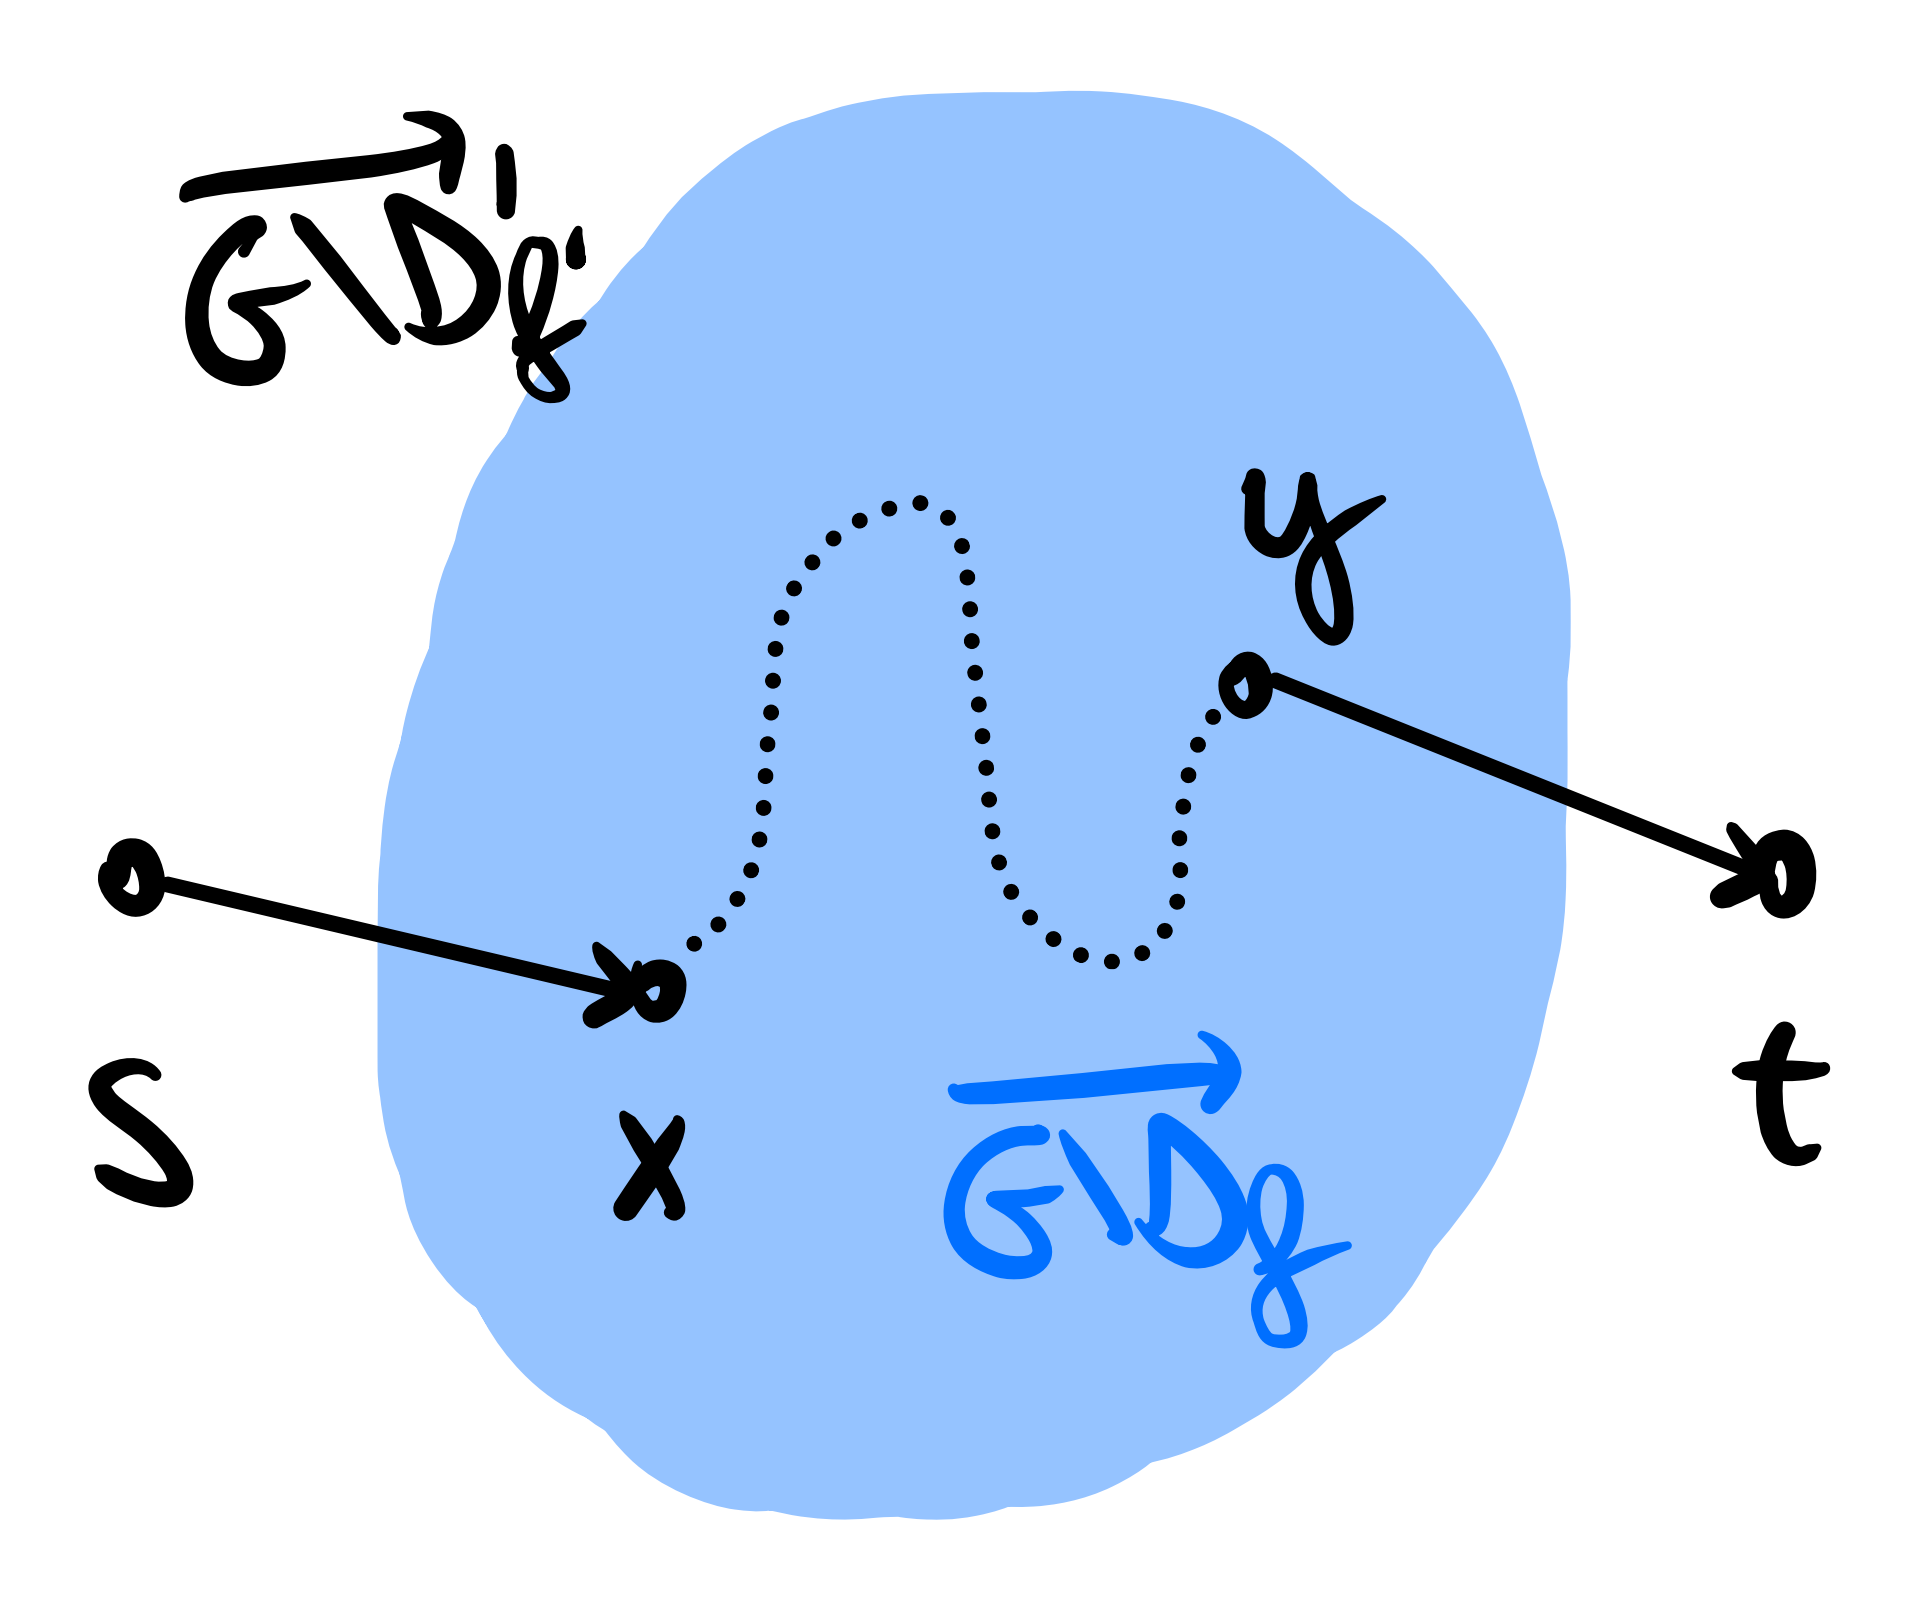
\includegraphics[width=\textwidth]{assignments/figures/resflowgraph.png}
% \caption{Schematic illustration of the residual flow graph with vertex $x \in V$ such that $(\mB\vf - \vd)(x) > 0$ and vertex $y \in V$ such that $(\mB\vf - \vd)(y) < 0$.}\label{fig:1:A:1:1}
% \end{marginfigure}

% Next, consider the levels of the sink $t$ in $\altflowgraph$ during each of the iterations $0 < i \leq h$. We write $\vf_i'$ for the flow obtained in the $i$-th iteration of Dinic's algorithm. By construction of $\altflowgraph$, we have that before any iteration of Dinic's algorithm, the shortest $s$-$t$ path has length $2$, so, $\ell_{\altflowgraph_{\vf_0'}}(t) \geq 2$.

% Using that the level of the sink vertex strictly increases during each iteration of Dinic's algorithm\footnote{Lemma 12.3.1 of the lecture notes.} and a simple induction on the number of iterations $i$, \begin{align*}
%     \ell_{\altflowgraph_{\vf_i'}}(t) \geq \ell_{\altflowgraph_{\vf_{i-1}'}}(t) + 1 \geq \ell_{\altflowgraph_{\vf_0'}}(t) + i \geq i + 2.
% \end{align*}

% Finally, consider the final flow $\vf' = \vf_h'$ and suppose for a contradiction that there exists an $x$-$y$ path $P$ in $\resflowgraph$ consisting of fewer than $h$ edges. Then. by our previous argument, $(s,x) + P + (y,t)$ is an $s$-$t$ path in $\altresflowgraph$ consisting of fewer than $h + 2$ edges. But this contradicts $\ell_{\altflowgraph_{\vf'}}(t) \geq h + 2$.
% \end{proof}

% \begin{thm}
% The expected running time of the flow procedure is at most $\TildeLandauO{\nicefrac{|D|}{\phi^2}}$.
% \end{thm}
% \begin{proof}
% We will prove the following two claims.

% \begin{clm}\label{clm:1:A:2:1}
% \textsc{FindBlockingFlow} (and therefore each iteration of Dinic's algorithm) takes expected time $\TildeLandauO{\norm{\vDelta}_1}$.
% \end{clm}
% \begin{clm}\label{clm:1:A:2:2}
% $\norm{\vDelta}_1 \leq \frac{4|D|}{\phi}$.
% \end{clm}

% \begin{rmk}
% It is important to note that at no point we fully construct the flow instance $\flowinstance$. That is, we do never construct the entire residual graph nor its level graph. Instead, we construct the parts of these graphs that are needed as we need them.
% \end{rmk}

% Using the two claims, running Dinic's algorithm for $h$ iterations takes expected time, \begin{align*}
%     \TildeLandauO{h \norm{\vDelta}_1} = \TildeLandauO{\frac{\Delta_{\max}(G)}{\phi} \cdot \frac{|D|}{\phi}} = \TildeLandauO{\frac{|D|}{\phi^2}}. \margintag{using $\Delta_{\max}(G) = \LandauO{1}$} &\qedhere
% \end{align*}
% \end{proof}

% \begin{cor}\label{cor:supply_bound}
% $\norm{\vDelta}_1 < \frac{n}{2} < \norm{\vnabla}_1 = n$
% \end{cor}
% \begin{proof}
% Using the assumption $|D| < \nicefrac{\phi n}{8}$, this is an immediate corollary of \cref{clm:1:A:2:2}.
% \end{proof}

% \begin{proof}[Proof of \cref{clm:1:A:2:1}]
% In the following, we denote the level graph with respect to which we want to find a blocking flow by $L$. We implement \textsc{FindBlockingFlow} using link-cut trees almost identically to the lecture notes. The only small adjustment we make is that we do not initialize the link-cut tree on all edges of the level graph, but add edges only when they are ``reached''.

% Recall that we used the procedure \textsc{Transform($L$)} to transform the level graph into a graph where each edge $e = (u,v)$ is replaced by a vertex $m$ incident to its two endpoints; the endpoints $u$ and $v$ receive cost $\infty$, and the vertex $m$ receives cost $\vc'(e)$. We write $L' \defeq \textsc{Transform}(L)$. As mentioned in the previous remark, we do not construct $L'$ explicitly, but will refer to its parts (i.e., vertices and their neighborhood) as we need them. Clearly, each particular vertex and neighborhood can be constructed in time $1 + \Delta_{\max}(G) = \LandauO{1}$.

% We define the operation \textsc{LC-Tree.AddEdge} receiving an already existing vertex $u$ and a vertex $v$ to be added with cost $\cost(v)$ as follows.

% \begin{algorithm}[H]
%     \caption{\textsc{LC-Tree.AddEdge($u, v$)}}
%     \textsc{LC-Tree.AddVertex}($v$)\;
%     \textsc{LC-Tree.AddCost($v, \cost(v)$)}\;
%     \textsc{LC-Tree.Link($u, v$)}\;
% \end{algorithm}

% Note that as $v$ is initially isolated, the cost-operation will not affect any other vertices. \textsc{FindBlockingFlow} is described in \cref{alg:1:A:1}. There, $H$ tracks all parts of the level graph that have been explored,\footnote{In a way (though not quite), $H$ corresponds to the complement of $H$ as used in the definition of \textsc{FindBlockingFlow} in the lecture notes.} thus if the neighborhood of $s$ in $H$ is identical to the neighborhood of $s$ in $L'$ the algorithm terminates. If this is not true, then we find an edge in the level graph that is not (and was not previously) in the link-cut tree and add it.

% \begin{algorithm}
%     \caption{\textsc{FindBlockingFlow($s, t, L$)}}\label{alg:1:A:1}
%     % $L' \gets \textsc{Transform}(L)$\;
%     $\textsc{LC-Tree} \gets \textsc{Initialize}(\emptyset)$\;
%     $\textsc{LC-Tree.AddVertex}(s)$\;
%     Let $H$ be an empty graph on vertices $V \cup \{s,t\}$\;
%     \While{$\vdeg_H(s) < \vdeg_{L'}(s)$}{
%         $u \gets \textsc{LC-Tree.FindRoot}(s)$\;
%         \uIf{$u = t$}{
%             $(w, c) \gets \textsc{LC-Tree.FindMin}(s)$\;
%             $\textsc{LC-Tree.AddCost}(s, -c)$\;
%             Add to $H$ and $\textsc{LC-Tree}$ (via $\textsc{Cut}(\cdot)$) all edges incident to $w$\;
%         }
%         \uElseIf{there is an edge $(u,v) \in L'$ such that $(u,v)$ is not in $\textsc{LC-Tree}$ and $(u,v) \not\in H$}{
%             $\textsc{LC-Tree.AddEdge}(u,v)$\;
%         }
%         \Else{
%             Add to $H$ and $\textsc{LC-Tree}$ (via $\textsc{Cut}(\cdot)$) all edges incident to $u$\;
%         }
%     }
%     Construct the blocking flow $\hat{\vf'}$ by setting for each edge $(u,v)$ of $L$, with mid-point $m$ in $L'$, the flow to equal $\cost(m)$ minus the cost on $m$ just before it was added to $H$\;
% \end{algorithm}

% Observe that \textsc{FindBlockingFlow} behaves analogously to the procedure defined in the lecture notes, except that vertices and edges are added lazily using the operation \textsc{LC-Tree.AddEdge}. It therefore follows immediately that the algorithm is correct and $\hat{\vf'}$ is indeed a blocking flow of the level graph $L$.

% It remains to show that the runtime of the procedure is at most $\TildeLandauO{\norm{\vDelta}_1}$. We distinguish two cases. First, consider the case where the shortest $s$-$t$ path in $L$ has length two, that is, there exists some vertex $v \in V$ with edges $(s,v)$ and $(v,t)$ in $L$. Note that $\vDelta \in \Nat_0^n$, implying that there are at most $\norm{\vDelta}_1$ vertices $v$ with edge $(s,v)$ in $L$. The only outgoing edge of such a vertex $v$ in the level graph is the edge $(v,t)$. Therefore, we add $\LandauO{\norm{\vDelta}_1}$ many vertices to the link-cut tree.

% Now, consider the case where the shortest $s$-$t$ path in $L$ has a length greater than two. We know that for any vertex $v \in V$ that does not have edge $(v,t)$ in the level graph, it must send $\vnabla(v) = 1$ units of flow to $t$. As the flow is upper bounded by $\norm{\vDelta}_1$, there can be at most $\norm{\vDelta}_1$ such ``internal'' vertices. Moreover, we know that the out-degree in $L$ of any vertex $v \in V$ is at most $\Delta_{\max}(G) = \LandauO{1}$. Therefore, we add $\LandauO{\norm{\vDelta}_1}$ many vertices to the link-cut tree.

% Using that each operation on the link-cut tree takes amortized time $\LandauO{\log^2 n}$, the statement follows.
% \end{proof}

% \begin{proof}[Proof of \cref{clm:1:A:2:2}]
% We have, \begin{align*}
%     \norm{\vDelta}_1 &= 4 \norm{\vdeg_{\invembed}}_1 \\
%     &= 8 \cdot |\invembed| \margintag{using the handshaking lemma, $\norm{\vdeg_E}_1 = 2|E|$} \\
%     &\leq 8 \cdot \conge(\embed) \cdot |D|,
% \intertext{as in the worst case, every edge in $D$ has congestion $\conge(\embed)$ and each is contributing path $\embed(e)$ is the embedding of a different edge $e \in H$. Using $\conge(\embed) \leq \nicefrac{1}{2\phi}$,}
%     &\leq \frac{4|D|}{\phi}. \qedhere
% \end{align*}
% \end{proof}

% \subsection{Part B: Implementing the Certify Outcome}
% We now consider the case where the flow $\vf$ satisfies the if-condition, $\mB\vf \leq \vd$.

% \begin{thm}
% $H'$ as returned by the algorithm is a $\nicefrac{1}{8}$-expander.
% \end{thm}
% \begin{proof}
% Consider any cut $\cut$ with $|S| \leq |\Bar{S}|$. As $H$ is a $\nicefrac{1}{2}$-expander, we have $|E_H\cut| \geq \nicefrac{|S|}{2}$. We will consider two cases.

% First, if $|E_{H'}\cut| \geq \nicefrac{|E_H\cut|}{4}$ (that is, ``few edges are removed from the cut''), we immediately obtain that $H'$ is a $\nicefrac{1}{8}$-expander, as we have, \begin{align*}
%     |E_{H'}\cut| \geq \frac{|E_H\cut|}{4} \geq \frac{|S|}{8},
% \end{align*} using that $H$ is a $\nicefrac{1}{2}$-expander.

% \begin{marginfigure}[7\baselineskip]
% 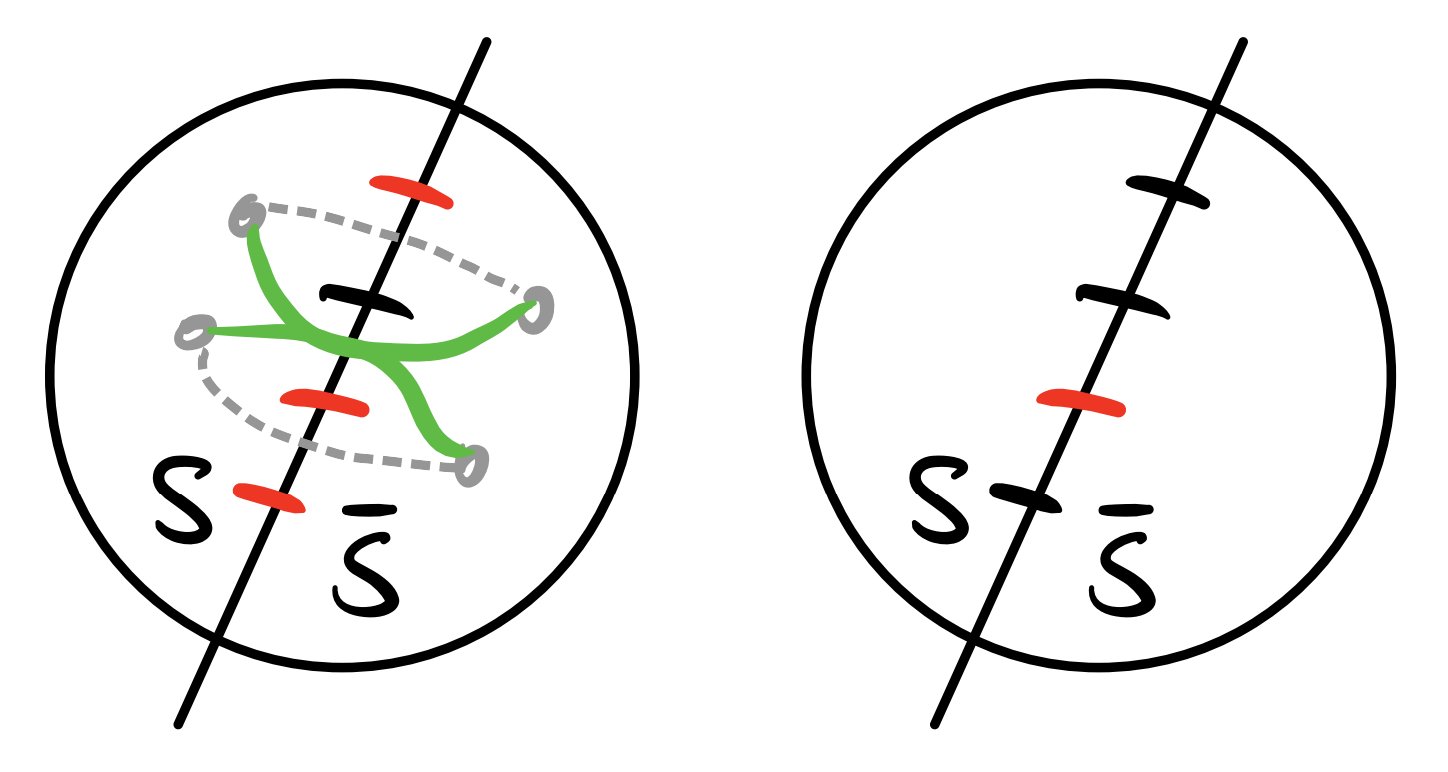
\includegraphics[width=\textwidth]{assignments/figures/cuts.png}
% \caption{Schematic illustration of the two cases. If not too many edges were removed, the graph is still an expander. If many edges were removed, the path decomposition leads to the addition of sufficiently many new edges.}
% \end{marginfigure}

% Now, suppose that $|E_{H'}\cut| < \nicefrac{|E_H\cut|}{4}$, that is, ``many edges are removed from the cut''. We will show that this implies that a sufficient amount of flow ``escapes'' the set $S$, yielding a sufficient number of edges to be added to $H'$ based on the flow path decomposition $\pathdecomp$. First, observe that if $F$ units of flow are transported from $S$ to $\Bar{S}$ (``across the cut''), then $|E_{\pathdecomp}\cut| \geq F$, as each vertex $v \in V$ can absorb at most $\vnabla(v) = 1$ units of flow. For the same reason, we know that, \begin{align*}
%     F \geq \trans{\vOne_S}\vDelta - \trans{\vOne_S}\vnabla = \trans{\vOne_S}\vDelta - |S|.
% \end{align*} Hence, it suffices to show that $\trans{\vOne_S}\vDelta \geq \frac{9}{8}|S|$, as then at least $\trans{\vOne_S}\vDelta - |S| \geq \nicefrac{|S|}{8}$ edges across the cut are added to $H'$ due to the flow path decomposition.

% Because for every removed cut-edge $\{u,v\}$ where $u \in S, v \in \Bar{S}$, $\vdeg_{\invembed}(u)$ increases by one, \begin{align*}
%     \trans{\vOne_S}\vDelta = 4 \cdot \trans{\vOne_S}\vdeg_{\invembed} &\geq 4\parentheses*{|E_H\cut| - |E_{H \setminus \invembed}\cut|} \\
%     &\geq 4\parentheses*{|E_H\cut| - |E_{H'}\cut|} \margintag{using $|E_{H \setminus \invembed}\cut| \leq |E_{H'}\cut|$} \\
%     &> 3 |E_H\cut| \margintag{using $|E_{H'}\cut| < \frac{|E_H\cut|}{4}$} \\
%     &\geq \frac{3}{2}|S| \margintag{using $|E_H\cut| \geq \frac{|S|}{2}$} \qedhere
% \end{align*}
% \end{proof}

% \begin{thm}
% $\GmD$ is a $\TildeLandauOmega{\phi}$-expander.
% \end{thm}
% \begin{proof}
% We will prove the following claim.

% \begin{clm}\label{clm:1:B:2:1}
% $\newembed$ has congestion at most $\TildeLandauO{\nicefrac{1}{\phi}}$.
% \end{clm}

% Now, consider any cut $\cut$ with $|S| \leq |\overline{S}|$. Since $H'$ is a $\LandauOmega{1}$-expander, we have that $|E_{H'}\cut| = \LandauOmega{|S|}$. From $\newembed$, we know that for each $\{u,v\} \in E_{H'}\cut$, we can find a $u$-$v$ path in $\GmD$ that has to cross the cut $\cut$ at least once. By the given claim, each edge in $\GmD$ is on at most $\TildeLandauO{\nicefrac{1}{\phi}}$ such paths, so at least $\TildeLandauOmega{\phi}|E_{H'}\cut| = \TildeLandauOmega{\phi |S|}$ edges in $\GmD$ cross the cut $\cut$.\footnote{This proof is analogous to the proof of lemma 14.2.1 of the lecture notes.}
% \end{proof}

% \begin{proof}[Proof of \cref{clm:1:B:2:1}] We write $H_1' \defeq H \setminus \invembed$ and $H_2'$ for the edges $\{u,v\}$ in $H'$ resulting from a $u$-$v$ path $\ora{\pi}$ from the flow path decomposition $\pathdecomp$. We write $\newembedOne$ and $\newembedTwo$ for the embedding $\newembed$ restricted to $H_1'$ and $H_2'$, respectively. Note that $H' = H_1' \cup H_2'$ and $\newembed = \newembedOne \cup \newembedTwo$. Thus, it is sufficient to show that both $\newembedOne$ and $\newembedTwo$ have congestion at most $\TildeLandauO{\nicefrac{1}{\phi}}$.

% Recall that, by assumption, the congestion of $\embed$ (and therefore also $\newembedOne$) is at most $\nicefrac{1}{2\phi} = \LandauO{\nicefrac{1}{\phi}}$.

% Finally, due to our choice of the edge capacities of the flow problem $\flowinstance$, each edge can be used by at most $C$ many paths of $\pathdecomp$, as every $u$-$v$ path transports at least, \begin{align*}
%     \min\{\vDelta(u), C, \vnabla(v)\} \geq \min\{4, C, 1\}, \margintag{using that $\vDelta(u) > 0$, as ``some'' flow is transported away from $u$}
% \end{align*} units of flow.\footnote{Since the edge capacity $C$ is integral (otherwise we cannot apply Dinic's algorithm); and any path flow must saturate at least one of its constituting edges.} Hence, the congestion of $\newembedTwo$ is at most, \begin{align*}
%     C = \frac{8 \Delta_{\max}(H)}{\phi} = \LandauO{\frac{\log^2 n}{\phi}} = \TildeLandauO{\frac{1}{\phi}},
% \end{align*} and the statement follows.
% \end{proof}

% \subsection{Part C: Implementing the Cut Outcome}
% Finally, we consider the case where the flow $\vf$ does not satisfy the if-condition, i.e., $\mB\vf \not\leq \vd$. We define the residual graph $\resflowgraph$ such that an edge $(u,v)$ is in the residual graph iff $(u,v)$ is not saturated by $\vf$. This ensures that the residual graph is simple.

% Let $S_0 \defeq \{v \in V \mid (\mB\vf - \vd)(v) > 0\}$ and for $i > 0$,\footnote{Note that the graphs are unweighted, so $\dist(u,v)$ corresponds to the length of the shortest $u$-$v$ path.} \begin{align}
%     S_i \defeq \{v \in V \mid \text{$\exists s \in S_0$ with $\dist_{\resflowgraph}(s,v) \leq i$}\}.
% \end{align} Observe that because the if-condition is not satisfied, $S_0 \neq \emptyset$. Letting $k$ be the number of iteration of the while-loop, observe that for $0 < i \leq k$, the sets $S_i$ coincide with the set $S$ after the $i$-th iteration of the while-loop. In particular, the set $S_k$ is returned by the algorithm.

% \begin{lem}
% For each $0 \leq i < k$, \begin{align}
%     \vol_{\resflowgraph}(S_{i+1}) \geq \parentheses*{1 + \frac{\phi}{8 \Delta_{\max}(G)}} \vol_{\resflowgraph}(S_i).
% \end{align}
% \end{lem}
% \begin{proof}
% Due to the definition of the set $S_{i+1}$, we have, \begin{align}
%     \vol_{\resflowgraph}(S_{i+1}) \geq \vol_{\resflowgraph}(S_i) + |\ora{E}_{\resflowgraph}(S_i, \overline{S_i})|. \label{eq:lem6_ineq1}
% \end{align} This is because in each iteration of the while-loop we add all vertices to $S_{i+1}$ that have distance one to the set $S_i$, and each of these new vertices will contribute at least one to the volume.

% Recall that due to our definition of the residual graph, we have that $\ora{e} \in \ora{E}_{\resflowgraph}(S_i, \overline{S_i})$ iff $\vf(\ora{e}) < C$. Thus, \begin{align}
%     |\ora{E}_{\resflowgraph}(S_i, \overline{S_i})| &= |\{\ora{e} \in \ora{E}_{\flowgraph}(S_i, \overline{S_i}) \mid \vf(\ora{e}) < C\}| \nonumber\\
%     &= |E_{\flowgraph}(S_i, \overline{S_i})| - |\{\ora{e} \in \ora{E}_{\flowgraph}(S_i, \overline{S_i}) \mid \vf(\ora{e}) = C\}| \nonumber\\
%     &\geq |E_{\flowgraph}(S_i, \overline{S_i})| - \frac{\trans{\vOne}_{S_i}\vDelta}{C} \margintag{using that the number of saturated cut-edges is at most $\nicefrac{\trans{\vOne}_{S_i}\vDelta}{C}$ and the amount of flow leaving $S_i$ is at most its supply, $\trans{\vOne}_{S_i}\vDelta$} \nonumber\\
%     &= |E_{\GmD}(S_i, \overline{S_i})| - \frac{4 \trans{\vOne}_{S_i} \vdeg_{\invembed}}{C} \nonumber\\
%     &\geq \phi|S_i| - \frac{4 |S_i| \Delta_{\max}(H)}{C} \margintag{using the while-condition, $|E_{\GmD}(S_i, \overline{S_i})| \geq \phi|S_i|$, and $\invembed \subseteq H$} \nonumber\\
%     &= \phi|S_i| - \frac{1}{2}\phi|S_i| \nonumber\\
%     &= \frac{1}{2}\phi|S_i|. \label{eq:lem6_ineq2}
% \end{align} Finally, observe that, \begin{align}
%     \vol_{\resflowgraph}(S_i) &\leq 2\vol_{\GmD}(S_i) \margintag{using that $\resflowgraph$ is simple but may contain antiparallel edges} \nonumber\\
%     &= 2 \sum_{v \in S_i} \vdeg_{\GmD}(v) \nonumber\\
%     & \leq 2|S_i| \Delta_{\max}(G). \label{eq:lem6_ineq3}
% \end{align} Combining inequalities \cref{eq:lem6_ineq1}, \cref{eq:lem6_ineq2}, and \cref{eq:lem6_ineq3} yields the desired bound.\footnote{Even slightly better by a small constant factor.}
% \end{proof}

% \begin{lem}
% $k \leq h$.
% \end{lem}
% \begin{proof} We prove the statement by contradiction. Let $h' \geq h$. By the previous lemma and a simple induction, \begin{align*}
%     \vol_{\resflowgraph}(S_{h'}) &\geq \parentheses*{1 + \frac{\phi}{8\Delta_{\max}(G)}}^{h'} \vol_{\resflowgraph}(S_0) \\
%     &\geq \parentheses*{1 + \frac{\phi}{8\Delta_{\max}(G)}}^h \margintag{using that $S_0 \neq \emptyset$, $\vol_{\resflowgraph}(S_0) \geq 1$} \\
%     &\geq \parentheses*{1 + \frac{\phi}{16\Delta_{\max}(G)} + \parentheses*{\frac{\phi}{16\Delta_{\max}(G)}}^2}^h \margintag{using $\phi \leq \Delta_{\max}(G)$ from the definition of sparsity} \\
%     &> e^{\frac{h\phi}{16\Delta_{\max}(G)}} \margintag{using $e^x < 1 + x + x^2$ for $0 < x \leq 1$} \\
%     &= e^{\log(4m)} = 4m,
% \end{align*} contradicting, \begin{align*}
%     \vol_{\resflowgraph}(S_{h'}) \leq 2\vol_G(S_{h'}) = 2 \sum_{v \in S_{h'}} \vdeg_G(v) \leq 4m. &\qedhere
% \end{align*}
% \end{proof}

% \begin{thm}
% $|S_k| \leq |\overline{S_k}|$ and $|E_{\GmD}(S_k,\overline{S_k})| < \phi|S_k|$.\footnote{Hence, $(S_k, \overline{S_k})$ is a $\phi$-sparse cut.}
% \end{thm}
% \begin{proof}
% Observe that $|E_{\GmD}(S_k,\overline{S_k})| < \phi|S_k|$ follows immediately because the set $S_k$ corresponds to the set after the final iteration of the while-loop, implying that the wile-condition is dissatisfied for $S_k$.

% \begin{clm}\label{clm:1:C:3:1}
% $|S_h| \leq \norm{\vDelta}_1$.
% \end{clm}

% Using this claim, we obtain, \begin{align*}
%     |S_k| \leq |S_h| \leq \norm{\vDelta}_1 \leq \frac{n}{2}. \margintag{using $S_k \subseteq S_h$ as $k \leq h$ and $\norm{\vDelta}_1 \leq \frac{n}{2}$ by \cref{cor:supply_bound}} &\qedhere
% \end{align*}
% \end{proof}

% \begin{proof}[Proof of \cref{clm:1:C:3:1}]
% By \cref{lem:1:A:1}, there is no vertex $y$ with $(\mB\vf - \vd)(y) < 0$ in $S_h$. Therefore, $|S_h|$ ``consumes'' at least $\trans{\vOne}_{S_h}\vnabla = |S_h|$ units of flow. However, note that there is at most $\norm{\vDelta}_1$ units of flow in total, and hence, we must have that $|S_h| = \trans{\vOne}_{S_h}\vnabla \leq \norm{\vDelta}_1$.
% \end{proof}

% \section{An $\ell_1$-Interior Point Method for Maximum Flow}

% \paragraph{Setting} We consider an undirected graph $G = (V,E)$ with capacities $\vc \in \Nat^{|E|}$. We write $n \defeq |V|, m \defeq |E|$, and assume $m > 10$ and $\norm{\vc}_1 \leq m^{10}$. Let $s, t \in V$ be some source and sink vertex. We assume that we are given the maximum $s$-$t$ flow value $0 < F \leq m^{10}$, which we assume to be integral.

% In the following, we will consider the graph $\Tilde{G} = (V, \Etil)$ where $\Etil \defeq E \cup \{\etil\}$ and $\etil = \{s,t\}$ is an edge with unlimited capacity. We assign an arbitrary orientation to edges $E$ and orient the edge $\etil$ such that its tail is $s$ and its head is $t$. Let $\mB$ be the incidence matrix of $\Tilde{G}$.

% We are interested in finding an $s$-$t$ flow $\vf \in \R^{|E|}$ with value $F$. We will do so by considering $s$-$t$ flows $\vf \in \R^{|\Etil|}$ that do not send any flow from $s$ to $t$ on edge $\etil$, i.e., $\vf(\etil) \leq 0$. We obtain the program, \begin{align}
%     \min_{\substack{\vf \in \R^{|\Etil|} \\ \mB\vf = F(\vOne_t - \vOne_s) \\ \forall e \in E \colon -\vc(e) \leq \vf(e) \leq \vc(e)}} \vf(\etil). \label{eq:2:program}
% \end{align}

% \paragraph{Barrier Program} We now consider a variant of the above program using barrier functions. Let, \begin{align*}
%     \barrierflowset \defeq \{\vf \in \R^{|\Etil|} \mid \text{$\vf(\etil) > 0$ and $\forall e \in E \colon -\vc(e) < \vf(e) < \vc(e)$}\},
% \end{align*} be a capacity-constrained flow set. We define a barrier $B: \barrierflowset \to \R$ by, \begin{align*}
%     B(\vf) \defeq \sum_{e \in E} - \log\parentheses*{1 - \frac{\vf(e)}{\vc(e)}} - \log\parentheses*{1 + \frac{\vf(e)}{\vc(e)}},
% \end{align*} and a potential function $\Phi : \barrierflowset \to \R$, $\Phi(\vf) \defeq 10 m \log(\vf(\etil)) + B(\vf)$. The \emph{barrier program} is described by, \begin{align}
%     \min_{\substack{\vf \in \barrierflowset \\ \mB\vf = F(\vOne_t - \vOne_s)}} \Phi(\vf). \label{eq:2:barrier_program}
% \end{align}

% \subsection{Part A: The Potential Function: Initialization and End-Goal}

% \begin{lem}
% Program \eqref{eq:2:program} is convex.
% \end{lem}
% \begin{proof}
% This immediately follows because the objective is linear, the equality constraint is linear, and the inequality constraints are linear (hence, convex).
% \end{proof}

% \begin{lem}
% The potential function $\Phi$ is non-convex.
% \end{lem}
% \begin{proof}
% Observe that $\Phi$ is twice continuously differentiable. We have for its gradient, \begin{align}
%     \grad \Phi(\vf)(e) = \begin{cases}
%         \frac{10 m}{\vf(\etil)} & e = \etil \\
%         \frac{1}{\vc(e) - \vf(e)} - \frac{1}{\vc(e) + \vf(e)} & e \in E, \\
%     \end{cases} \label{eq:2:gradient}
% \end{align} and for its (diagonal!) Hessian, \begin{align}
%     \mH_\Phi(\vf)(e,e) = \begin{cases}
%         -\frac{10 m}{\vf(\etil)^2} & e = \etil \\
%         \frac{1}{(\vc(e) - \vf(e))^2} + \frac{1}{(\vc(e) + \vf(e))^2} & e \in E. \\
%     \end{cases} \label{eq:2:hessian}
% \end{align} Clearly, $\mH_\Phi(\vf)$ is not positive semi-definite, and hence, by the second-order characterization of convexity, $\Phi$ is non-convex.
% \end{proof}

% \begin{cor}
% Program \eqref{eq:2:barrier_program} is non-convex.
% \end{cor}

% \begin{lem}
% Any optimal solution $\s{\vf}$ for the program \eqref{eq:2:program} routes $F$ units of flow from $s$ to $t$ on the edges of $E$ and has $\s{\vf}(\etil) = 0$.
% \end{lem}
% \begin{proof}
% Due to the definition of $F$, there exists a flow $\vf \in \R^{|E|}$ routing $F$ units of flow from $s$ to $t$. By definition, $\vf$ only uses the edges of $E$. This implies that $\s{\vf}(\etil) \leq 0$.

% Now suppose that $\s{\vf}(\etil) < 0$. But then, the flow $\vf$ defined by $\vf(e) \defeq \s{\vf}(e)$ for $e \in E$ and $\vf(\etil) = 0$ routes $F - \s{\vf}(\etil) > F$ units of flow from $s$ to $t$, contradicting the definition of $F$.
% \end{proof}

% \begin{lem}[Termination]\label{lem:termination}
% If $\vf \in \barrierflowset$ and $\Phi(\vf) \leq -10 m \log m$,\footnote{The assumption $\mB\vf = F(\vOne_t - \vOne_s)$ is not needed here.} then $\vf(\etil) \leq \nicefrac{1}{m}$.\footnote{So $\vf$ is an approximate solution to program \eqref{eq:2:program}.}
% \end{lem}
% \begin{proof}
% As $\vf \in \barrierflowset$, we know that $\nicefrac{\vf(e)}{\vc(e)} \in (-1,1)$. We write $\vDelta(e) \defeq |\nicefrac{\vf(e)}{\vc(e)}| \in [0,1)$. Because the logarithm is concave, we have that $|\log(1-\vDelta(e))| > |\log(1+\vDelta(e))|$. We also have that $\log(1-\vDelta(e)) < 0$ and $\log(1+\vDelta(e)) > 0$. This shows that $B(\vf) \geq 0$.

% As we assumed $\Phi(\vf) \leq -10 m \log m$, this implies, \begin{align*}
%     && 10 m \log(\vf(\etil)) &\leq -10 m \log m \\
%     \implies&& \log(\vf(\etil)) &\leq \log\parentheses*{\frac{1}{m}} \\
%     \implies&& \vf(\etil) &\leq \frac{1}{m}. \qedhere
% \end{align*}
% \end{proof}

% \begin{lem}[Initialization]\label{lem:initialization}
% For $\vf_0 \defeq F\vOne_{\etil}$, we have $\mB\vf_0 = F(\vOne_t - \vOne_s)$, $\vf_0 \in \barrierflowset$, and $\Phi(\vf_0) \leq 100 m \log m$.
% \end{lem}
% \begin{proof}
% \begin{enumerate}
%     \item We have $\mB\vf_0 = F\mB\vOne_{\etil} = F(\vOne_t - \vOne_s)$ per the definition of the orientation of $\etil$.
%     \item We have $\vf_0(\etil) = F > 0$ and we have that for any $e \in E$, \begin{align*}
%         \vf_0(e) = 0 \in (-\vc(e), \vc(e)),
%     \end{align*} so $\vf_0 \in \barrierflowset$.
%     \item Observe that $B(\vf_0) = \sum_{e \in E} - 2 \log(1) = 0$. We have, \begin{align*}
%         \Phi(\vf_0) &= 10 m \log(\vf_0(\etil)) + B(\vf_0) \\
%         &= 10 m \log(F) \\
%         &\leq 10 m \log(m^{10}) \margintag{using that the sum of capacities is at most $m^{10}$} \\
%         &= 100 m \log m. \qedhere
%     \end{align*}
% \end{enumerate}
% \end{proof}

% \subsection{Part B: IPM Progress using Updates}

% Given $\vf \in \barrierflowset$, we define $\vl \in \R^{|\Etil|}$ by $\vl(\etil) \defeq \nicefrac{1}{\vf(\etil)}$ and \begin{align*}
%     \vl(e) \defeq \frac{1}{\min\{\vc(e) - \vf(e), \vc(e) + \vf(e)\}}
% \end{align*} for all $e \in E$. Observe that $\vl_\vf > \vZero$ (in each coordinate) as $\vf(\etil) > 0$ and $\vf(e) \in (-\vc(e), \vc(e))$ for all $e \in E$. We define a corresponding diagonal matrix $\mL_\vf \defeq \diag_{e \in \Etil}(\vl_\vf(e))$.

% In the following we will consider ``updates'' (that is, circulations\footnote{A circulation is a flow $\vdelta$ satisfying $\mB\vdelta = \vZero$.}) $\vdelta \in \R^{|\Etil|}$.

% \begin{lem}
% If $\norm{\mL_\vf \vdelta}_\infty \leq \nicefrac{1}{2}$, then $\vf + \vdelta \in \barrierflowset$.
% \end{lem}
% \begin{proof}
% \begin{enumerate}
%     \item By assumption, $|\vl_\vf(\etil) \cdot \vdelta(\etil)| = \vl_\vf(\etil) \cdot |\vdelta(\etil)| \leq \nicefrac{1}{2}$. This implies $|\vdelta(\etil)| \leq \nicefrac{1}{2 \vl_\vf(\etil)} = \nicefrac{\vf(\etil)}{2}$. From this, we get, \begin{align*}
%         \vf(\etil) + \vdelta(\etil) \geq \vf(\etil) - \frac{\vf(\etil)}{2} = \frac{\vf(\etil)}{2} > 0.
%     \end{align*}
%     \item Fix any $e \in E$. By assumption, $|\vl_\vf(e) \cdot \vdelta(e)| = \vl_\vf(e) \cdot |\vdelta(e)| \leq \nicefrac{1}{2}$. Consider two cases: \begin{enumerate}[label=(\roman*)]
%         \item If $\vf(e) \geq 0$, then $\vl_\vf(e) = \frac{1}{\vc(e) - \vf(e)}$, implying, $|\vdelta(e)| \leq \frac{\vc(e) - \vf(e)}{2}$. Thus, \begin{align*}
%             \vf(e) + \vdelta(e) &\leq \vf(e) + \frac{\vc(e) - \vf(e)}{2} = \frac{\vf(e) + \vc(e)}{2} < \vc(e) \quad\text{and} \margintag{using $\vf(e) < \vc(e)$} \\
%             \vf(e) + \vdelta(e) &\geq \vf(e) - \frac{\vc(e) - \vf(e)}{2} \\
%             &= \frac{3\vf(e) - \vc(e)}{2} \geq -\frac{\vc(e)}{2} > -\vc(e). \margintag{using $\vf(e) \geq 0$}
%         \end{align*}
%         \item If $\vf(e) < 0$, then $\vl_\vf(e) = \frac{1}{\vc(e) + \vf(e)}$, implying, $|\vdelta(e)| \leq \frac{\vc(e) + \vf(e)}{2}$. Thus, \begin{align*}
%             \vf(e) + \vdelta(e) &\geq \vf(e) - \frac{\vc(e) + \vf(e)}{2} = \frac{\vf(e) - \vc(e)}{2} > -\vc(e) \quad\text{and} \margintag{using $\vf(e) > -\vc(e)$} \\
%             \vf(e) + \vdelta(e) &\leq \vf(e) + \frac{\vc(e) + \vf(e)}{2} \\
%             &= \frac{3\vf(e) + \vc(e)}{2} < \frac{\vc(e)}{2} < \vc(e). \margintag{using $\vf(e) < 0$}
%         \end{align*}
%     \end{enumerate}
% \end{enumerate}
% Altogether, we have $(\vf + \vdelta)(\etil) > 0$ and $(\vf + \vdelta)(e) \in (-\vc(e), \vc(e))$ for all $e \in E$, so $\vf + \vdelta \in \barrierflowset$.
% \end{proof}

% \begin{lem}\label{lem:2:B:2}
% If $\norm{\mL_\vf \vdelta}_\infty \leq \nicefrac{1}{2}$, then \begin{align}
%     \Phi(\vf + \vdelta) \leq \Phi(\vf) + \trans{\grad \Phi(\vf)}\vdelta + 4 \norm{\mL_\vf \vdelta}_1^2.
% \end{align}
% \end{lem}
% \begin{proof}
% We have seen that $\vf + \vdelta \in \barrierflowset$, so $\Phi(\vf + \vdelta)$ is well-defined. By Taylor's theorem (second-order form), \begin{align}
%     \Phi(\vf + \vdelta) = \Phi(\vf) + \trans{\grad\Phi(\vf)}\vdelta + \frac{1}{2}\trans{\vdelta}\mH_\Phi(\vftil)\vdelta, \label{eq:2:B:1:1}
% \end{align} where $\vftil \defeq (1-\theta)\vf + \theta(\vf + \vdelta) = \vf + \theta\vdelta$ for some $\theta \in [0,1]$. We have, \begin{align*}
%     &\trans{\vdelta}\mH_\Phi(\vf + \theta\vdelta)\vdelta \\
%     &= \begin{multlined}[t]
%         -10 m \frac{\vdelta(\etil)^2}{(\vf(\etil) + \theta\vdelta(\etil))^2} \\ + \sum_{e \in E} \parentheses*{\frac{1}{(\vc(e) - \vf(e) - \theta\vdelta(e))^2} + \frac{1}{(\vc(e) + \vf(e) + \theta\vdelta(e))^2}}\vdelta(e)^2
%     \end{multlined} \margintag{using our characterization of $\mH_\Phi$ from \cref{eq:2:hessian}} \\
%     &\leq \sum_{e \in E} \parentheses*{\frac{1}{(\vc(e) - \vf(e) + \theta|\vdelta(e)|)^2} + \frac{1}{(\vc(e) + \vf(e) - \theta|\vdelta(e)|)^2}}\vdelta(e)^2.
% \intertext{From $\norm{\mL_\vf\vdelta}_\infty \leq \nicefrac{1}{2}$, we conclude that\begin{align*}
%     |\vdelta(e)| \leq \frac{1}{2 \vl_\vf(e)} = \frac{\min\{\vc(e) - \vf(e), \vc(e) + \vf(e)\}}{2}
% \end{align*} for all $e \in E$. This implies that $\frac{1}{(\vc(e) - \vf(e) + \theta|\vdelta(e)|)^2} \leq \frac{4}{(\vc(e) - \vf(e))^2}$ and similarly in the other case, $\frac{1}{(\vc(e) + \vf(e) - \theta|\vdelta(e)|)^2} \leq \frac{4}{(\vc(e) + \vf(e))^2}$, yielding,}
%     &\leq 4 \sum_{e \in E} \parentheses*{\frac{1}{(\vc(e) - \vf(e))^2} + \frac{1}{(\vc(e) + \vf(e))^2}}\vdelta(e)^2 \\
%     &\leq 8 \sum_{e \in E} \vl_\vf(e)^2\vdelta(e)^2 \margintag{using $\frac{1}{(\vc(e) - \vf(e))^2} + \frac{1}{(\vc(e) + \vf(e))^2} \leq 2\vl_\vf(e)^2$} \\
%     &\leq 8 \parentheses*{\sum_{e \in E} \vl_\vf(e)|\vdelta(e)|}^2 \margintag{using $\sum_{i=1}^n a_i^2 \leq \parentheses*{\sum_{i=1}^n a_i}^2$ if $a_i \geq 0$} \\
%     &= 8 \norm{\mL_\vf \vdelta}_1^2.
% \end{align*} Plugging this inequality into \cref{eq:2:B:1:1}, we obtain the desired bound.
% \end{proof}

% \begin{lem}[Update]\label{lem:update}
% If for some $\kappa > 1$, we have $\norm{\mL_\vf \vdelta}_1 \leq \kappa$ and $\trans{\grad \Phi(\vf)}\vdelta = -1$, then \begin{align}
%     \Phi\parentheses*{\vf + \frac{1}{8\kappa^2}\vdelta} \leq \Phi(\vf) - \frac{1}{16\kappa^2}.
% \end{align}
% \end{lem}
% \begin{proof}
% Let $\vdelta' \defeq \frac{1}{8\kappa^2}\vdelta$. We have, \begin{align*}
%     \norm{\mL_\vf\vdelta'}_\infty = \frac{1}{8\kappa^2}\norm{\mL_\vf\vdelta}_\infty \leq \frac{1}{8\kappa^2}\norm{\mL_\vf\vdelta}_1 \leq \frac{1}{8\kappa} \leq \frac{1}{2}. \margintag{using $\norm{\cdot}_\infty \leq \norm{\cdot}_1$ and $\norm{\mL_\vf\vdelta}_1 \leq \kappa$}
% \end{align*} Therefore, by \cref{lem:2:B:2}, \begin{align*}
%     \Phi(\vf + \vdelta') &\leq \Phi(\vf) + \trans{\grad \Phi(\vf)}\vdelta' + 4\norm{\mL_\vf\vdelta'}_1^2 \\
%     &= \Phi(\vf) + \frac{1}{8\kappa^2}\underbrace{\trans{\grad \Phi(\vf)}\vdelta}_{=-1} + \frac{1}{16\kappa^4}\underbrace{\norm{\mL_\vf\vdelta}_1^2}_{\leq \kappa^2} \\
%     &\leq \Phi(\vf) - \frac{1}{8\kappa^2} + \frac{1}{16\kappa^2} \\
%     &= \Phi(\vf) - \frac{1}{16\kappa^2}. \qedhere
% \end{align*}
% \end{proof}

% \subsection{Part C: The Update}

% Let us consider the \emph{update program}, \begin{align}
%     \min_{\substack{\vdelta \in \R^{|\Etil|} \\ \mB\vdelta = \vZero \\ \trans{\grad\Phi(\vf)}\vdelta = -1}} \norm{\mL_\vf \vdelta}_1, \label{eq:2:update_program}
% \end{align} given the current flow $\vf \in \barrierflowset$.

% \begin{lem}
% The update program \eqref{eq:2:update_program} is convex.
% \end{lem}
% \begin{proof}
% Observe that the two equality constraints are linear in $\vdelta$. It is therefore sufficient to show that the objective is convex.

% Fix any $\theta \in [0,1]$ and $\vx, \vy \in \R^{|\Etil|}$. We have, \begin{align*}
%     \norm{\mL_\vf (\theta\vx + (1-\theta)\vy)}_1 &= \norm{\theta \mL_\vf \vx + (1-\theta) \mL_\vf \vy}_1 \\
%     &\leq \norm{\theta \mL_\vf \vx}_1 + \norm{(1-\theta) \mL_\vf \vy}_1 \margintag{using the triangle inequality} \\
%     &= \theta\norm{\mL_\vf \vx}_1 + (1-\theta)\norm{\mL_\vf \vy}_1. \qedhere
% \end{align*}
% \end{proof}

% \begin{lem}
% Let $\s{\gamma}$ be the value of the update program \eqref{eq:2:update_program}. We have, $\s{\gamma} \leq 1$.\footnote{This is a slightly better constant than what we were asked for.}
% \end{lem}
% \begin{proof}
% Let $\s{\vf}$ be an optimal solution and $\vf$ be a feasible solution (that is not optimal) to program \eqref{eq:2:program} and let $\vdeltabar \defeq \alpha(\s{\vf} - \vf)$ where \begin{align*}
%     \alpha \defeq - \frac{1}{\trans{\grad\Phi(\vf)}(\s{\vf} - \vf)}
% \end{align*} and $\vf$ is chosen such that $\trans{\grad\Phi(\vf)}(\s{\vf} - \vf) \neq 0$.\footnote{Such an $\vf$ clearly exists, take $\vf_0$ for example.} We will first show that $\vdeltabar$ is a feasible solution for program \eqref{eq:2:update_program} and then see that $\norm{\mL_\vf\vdeltabar}_1 \leq 1$, implying $\s{\gamma} \leq 1$.

% We have, \begin{align*}
%     \mB\vdeltabar = \alpha(\mB\s{\vf} - \mB\vf) = \alpha(F(\vOne_t - \vOne_s) - F(\vOne_t - \vOne_s)) = \vZero, \margintag{using feasibility of $\s{\vf}$ and $\vf$ w.r.t. program \eqref{eq:2:program}}
% \end{align*} so $\vdeltabar$ is indeed a cycle flow. Moreover, \begin{align*}
%     \trans{\grad\Phi(\vf)}\vdeltabar = \alpha\trans{\grad\Phi(\vf)}(\s{\vf} - \vf) = -\frac{\trans{\grad\Phi(\vf)}(\s{\vf} - \vf)}{\trans{\grad\Phi(\vf)}(\s{\vf} - \vf)} = -1.
% \end{align*} This shows that $\vdeltabar$ is feasible.

% It remains to show that $\norm{\mL_\vf\vdeltabar}_1 \leq 1$. We will use the following two claims, which we will prove later.

% \begin{clm}\label{clm:2:C:2:1}
% For all $e \in E$, $\frac{\s{\vf}(e) - \vf(e)}{\vc(e) - \vf(e)} \leq 1 - \frac{|\s{\vf}(e) - \vf(e)|}{\vc(e) - \vf(e)}$.
% \end{clm}
% \begin{clm}\label{clm:2:C:2:2}
% For all $e \in E$, $-\frac{\s{\vf}(e) - \vf(e)}{\vc(e) + \vf(e)} \leq 1 - \frac{|\s{\vf}(e) - \vf(e)|}{\vc(e) + \vf(e)}$.
% \end{clm}

% Using our characterization of $\grad\Phi$ from \cref{eq:2:gradient}, we obtain, \begin{align*}
%     &\trans{\grad\Phi(\vf)}(\s{\vf} - \vf) \\
%     &= 10m\frac{\s{\vf}(\etil) - \vf(\etil)}{\vf(\etil)} + \sum_{e \in E} \parentheses*{\frac{1}{\vc(e) - \vf(e)} - \frac{1}{\vc(e) + \vf(e)}}\parentheses*{\s{\vf}(e) - \vf(e)} \\
%     &= -10m + \sum_{e \in E} \parentheses*{\frac{1}{\vc(e) - \vf(e)} - \frac{1}{\vc(e) + \vf(e)}}\parentheses*{\s{\vf}(e) - \vf(e)} \margintag{using $\s{\vf}(\etil) = 0$} \\
%     &\leq -8m - \sum_{e \in E} \parentheses*{\frac{1}{\vc(e) - \vf(e)} + \frac{1}{\vc(e) + \vf(e)}}|\s{\vf}(e) - \vf(e)|. \margintag{using \cref{clm:2:C:2:1} and \cref{clm:2:C:2:2}}
% \end{align*} Next, observe that, \begin{align*}
%     &\sum_{e \in E} \parentheses*{\frac{1}{\vc(e) - \vf(e)} + \frac{1}{\vc(e) + \vf(e)}}|\s{\vf}(e) - \vf(e)| \\
%     &\geq \sum_{e \in E} \vl_\vf(e) \cdot |\s{\vf}(e) - \vf(e)| \\
%     &= \norm{\mL_\vf(\s{\vf} - \vf)}_1 - \vl_\vf(\etil) \cdot |\s{\vf}(\etil) - \vf(\etil)| \\
%     &= \norm{\mL_\vf(\s{\vf} - \vf)}_1 - \frac{|\vf(\etil)|}{\vf(\etil)} \margintag{using $\s{\vf}(\etil) = 0$} \\
%     &\geq \norm{\mL_\vf(\s{\vf} - \vf)}_1 - 1.
% \end{align*} Combining the two inequalities, we obtain, \begin{align*}
%     \trans{\grad\Phi(\vf)}(\s{\vf} - \vf) \leq -8m - \norm{\mL_\vf(\s{\vf} - \vf)}_1 + 1 \leq -\norm{\mL_\vf(\s{\vf} - \vf)}_1.
% \end{align*} In particular, $\trans{\grad\Phi(\vf)}(\s{\vf} - \vf) < 0$, using that $\trans{\grad\Phi(\vf)}(\s{\vf} - \vf) \neq 0$. Altogether, we have, \begin{align*}
%     \norm{\mL_\vf\vdeltabar}_1 &= |\alpha|\norm{\mL_\vf(\s{\vf} - \vf)}_1 \\
%     &= \frac{\norm{\mL_\vf(\s{\vf} - \vf)}_1}{|\trans{\grad\Phi(\vf)}(\s{\vf} - \vf)|} \\
%     &= -\frac{\norm{\mL_\vf(\s{\vf} - \vf)}_1}{\trans{\grad\Phi(\vf)}(\s{\vf} - \vf)} \margintag{using $\trans{\grad\Phi(\vf)}(\s{\vf} - \vf) < 0$} \\
%     &\leq \frac{\norm{\mL_\vf(\s{\vf} - \vf)}_1}{\norm{\mL_\vf(\s{\vf} - \vf)}_1} \margintag{using $\trans{\grad\Phi(\vf)}(\s{\vf} - \vf) < -\norm{\mL_\vf(\s{\vf} - \vf)}_1$} \\
%     &= 1. \qedhere
% \end{align*}
% \end{proof}

% \begin{proof}[Proof of \cref{clm:2:C:2:1}]
% Fix any $e \in E$. We have, \begin{align*}
%     \frac{\s{\vf}(e) - \vf(e)}{\vc(e) - \vf(e)} &= \frac{\s{\vf}(e) - \vc(e) + \vc(e) - \vf(e)}{\vc(e) - \vf(e)} \\
%     &= 1 - \frac{|\s{\vf}(e) - \vc(e)|}{\vc(e) - \vf(e)} \margintag{using $\s{\vf}(e) - \vc(e) \leq 0$} \\
%     &\leq 1 - \frac{|\s{\vf}(e) - \vf(e)|}{\vc(e) - \vf(e)}. \margintag{using $|\vf(e)| \leq \vc(e)$} \qedhere
% \end{align*}
% \end{proof}

% \begin{proof}[Proof of \cref{clm:2:C:2:2}]
% Fix any $e \in E$. We have, \begin{align*}
%     -\frac{\s{\vf}(e) - \vf(e)}{\vc(e) + \vf(e)} &= -\frac{\s{\vf}(e) + \vc(e) - (\vc(e) + \vf(e))}{\vc(e) + \vf(e)} \\
%     &= 1 - \frac{|\s{\vf}(e) + \vc(e)|}{\vc(e) + \vf(e)} \margintag{using $\s{\vf}(e) + \vc(e) \geq 0$} \\
%     &\leq 1 - \frac{|\s{\vf}(e) - \vf(e)|}{\vc(e) + \vf(e)}. \margintag{using $|\vf(e)| \leq \vc(e)$} \qedhere
% \end{align*}
% \end{proof}

% \begin{lem}
% There exists an optimal solution $\s{\vdelta}$ for the update program \eqref{eq:2:update_program}, which is supported on a single cycle.
% \end{lem}
% \begin{proof}
% Let $\vdelta$ be a feasible solution for the update program. We will later prove the following claim.

% \begin{clm}\label{clm:2:C:3:1}
% Any circulation flow $\vdelta$ (i.e., $\mB\vdelta = \vZero$) can be decomposed into $k$ cycle flows $\vdelta_1, \dots, \vdelta_k$ (i.e., $\vdelta = \sum_{i=1}^k \vdelta_i$) such that the cycle flows\footnote{A cycle flow is a circulation flow that sends the same amount of flow on every edge in its support, that is, it is supported on a single cycle. In particular, any cycle flow $\vdelta$ satisfies $\mB\vdelta = \vZero$} send flow into the same direction on every edge. More formally, for all $e \in \Etil$ and $i,j \in [k]$, we have that either $\vdelta_i(e),\vdelta_j(e) \leq 0$ or $\vdelta_i(e),\vdelta_j(e) \geq 0$.
% \end{clm}

% Visually, this property corresponds to the fact that a drawing of $\vdelta_1, \dots, \vdelta_k$ does not have antiparallel edges. In the following, we will therefore call cycle decompositions obeying by this property \emph{parallel} and cycle flows mutually violating this property on some edge \emph{antiparallel}.

% Let $\vdelta_1, \dots, \vdelta_k$ be an parallel cycle decomposition of $\vdelta$. We know that $\trans{\grad\Phi(\vf)}\vdelta = -1$. Because this is a linear function in $\vdelta$, there must exist some cycle flow $\vdelta_j$ such that $\trans{\grad\Phi(\vf)}\vdelta_j \leq -1$. We define the cycle flow, \begin{align*}
%     \vdeltabar \defeq \alpha\vdelta_j, \quad\text{where}\quad \alpha = -\frac{1}{\trans{\grad\Phi(\vf)}\vdelta_j} = \frac{1}{|\trans{\grad\Phi(\vf)}\vdelta_j|} \leq 1.
% \end{align*} In particular, $\norm{\mL_\vf\vdeltabar}_1 \leq \norm{\mL_\vf\vdelta_j}_1$. We will show that $\vdeltabar$ is at least as ``good'' as $\vdelta$ w.r.t. the update program.

% First, observe that $\vdeltabar$ is a feasible solution as $\mB\vdeltabar = \alpha\mB\vdelta_j = \vZero$ and \begin{align*}
%     \trans{\grad\Phi(\vf)}\vdeltabar = \alpha\trans{\grad\Phi(\vf)}\vdelta_j = -1.
% \end{align*} We have, \begin{align*}
%     \norm{\mL_\vf\vdelta}_1 &= \sum_{e \in \Etil} \vl_\vf(e) \cdot |\vdelta(e)| \\
%     &= \sum_{e \in \Etil} \vl_\vf(e) \cdot \left|\sum_{i=1}^k \vdelta_i(e)\right| \\
%     &= \sum_{e \in \Etil} \vl_\vf(e) \cdot \parentheses*{\sum_{i=1}^k |\vdelta_i(e)|} \margintag{using that the cycle decomposition is parallel} \\
%     &= \sum_{i=1}^k \sum_{e \in \Etil} \vl_\vf(e) \cdot |\vdelta_i(e)| \\
%     &= \sum_{i=1}^k \norm{\mL_\vf\vdelta_i}_1 \\
%     &\geq \norm{\mL_\vf\vdelta_j}_1 \\
%     &\geq \norm{\mL_\vf\vdeltabar}_1. \margintag{using $\norm{\mL_\vf\vdeltabar}_1 \leq \norm{\mL_\vf\vdelta_j}_1$}
% \end{align*} In particular, given the optimal solution $\s{\vdelta}$, $\s{\vdeltabar}$ is also optimal.
% \end{proof}

% \begin{proof}[Proof of \cref{clm:2:C:3:1}]
% Let $\vdelta_1, \dots, \vdelta_k$ be any cycle decomposition of the circulation $\vdelta$ with $l > 0$ antiparallel pairs of mutually antiparallel cycle flows. We will give a procedure that yields a cycle decomposition $\vdelta_1', \dots, \vdelta_{k'}'$ with at most $l - 1$ mutually antiparallel cycle flows. Repeating this procedure at most $l$ times yields the desired cycle decomposition. We denote by, \begin{align*}
%     C_i \defeq \{e \in \Etil \mid |\vdelta_i(e)| > 0\},
% \end{align*} the support of the $i$-th cycle flow of the cycle decomposition.

% The procedure works as follows. Let $\vdelta_i,\vdelta_j$ be any pair of mutually antiparallel cycle flows on edges $\bar{E} \subseteq \Etil$. W.l.o.g. we assume $\vdelta_i(\bar{e}) > 0$, $\vdelta_j(\bar{e}) < 0$ for $\bar{e} \in \bar{E}$ and that $\vdelta_i$ and $\vdelta_j$ route $\alpha$ and $\beta$ units of flow, respectively. To simplify the presentation, we also assume $\alpha \geq \beta$, the other case is symmetric.

% \begin{marginfigure}[-3\baselineskip]
% 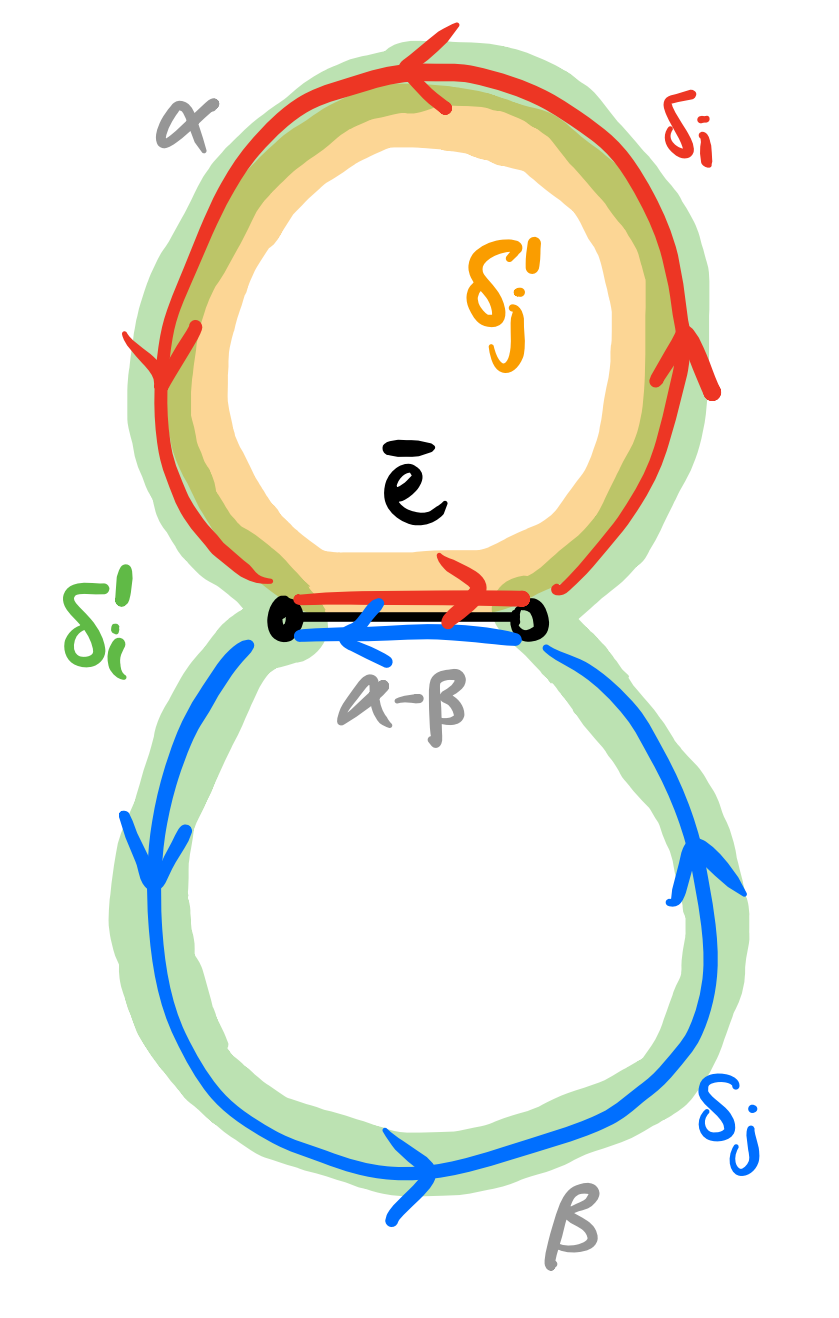
\includegraphics[width=\textwidth]{assignments/figures/cycle_decomposition.png}
% \caption{Schematic illustration of the cycle flow update. $\vdelta_i$ sends $\alpha$ units of flow and $\vdelta_j$ sends $\beta$ units of flow. The net flow on the edge $\bar{e}$ is $\alpha - \beta$.}\label{fig:2:C:3:1}
% \end{marginfigure}

% First, assume that $\vdelta_i$ and $\vdelta_j$ do not share any parallel edges. A schematic illustration is given in \cref{fig:2:C:3:1}. We define the cycle flows, \begin{align*}
%     \vdelta_i'(e) &\defeq \begin{cases}
%         \beta & e \in C_i \cup C_j \setminus \bar{E} \\
%         0 & \text{otherwise}, \\
%     \end{cases} \\
%     \vdelta_j'(e) &\defeq \begin{cases}
%         \alpha - \beta & e \in C_i \\
%         0 & \text{otherwise}. \\
%     \end{cases}
% \end{align*} Note that $\vdelta_j' = \vZero$ if $\alpha = \beta$.

% Clearly, $\vdelta_i' + \vdelta_j' = \vdelta_i + \vdelta_j$. Moreover, $\vdelta_i'$ and $\vdelta_j'$ are not mutually antiparallel, as any edge $\bar{e} \in \bar{E}$ where flow was sent into opposite directions is only in the support of $\vdelta_j'$ and on all edges in the shared support $C_i \setminus \bar{E}$ flow is sent into the same direction. Hence, the cycle decomposition, \begin{align*}
%     \vdelta_1, \dots, \vdelta_{i-1}, \vdelta_i', \vdelta_{i+1}, \dots, \vdelta_{j-1}, \vdelta_j', \vdelta_{j+1}, \dots, \vdelta_k,
% \end{align*} has the desired properties.

% \begin{marginfigure}[-3\baselineskip]
% 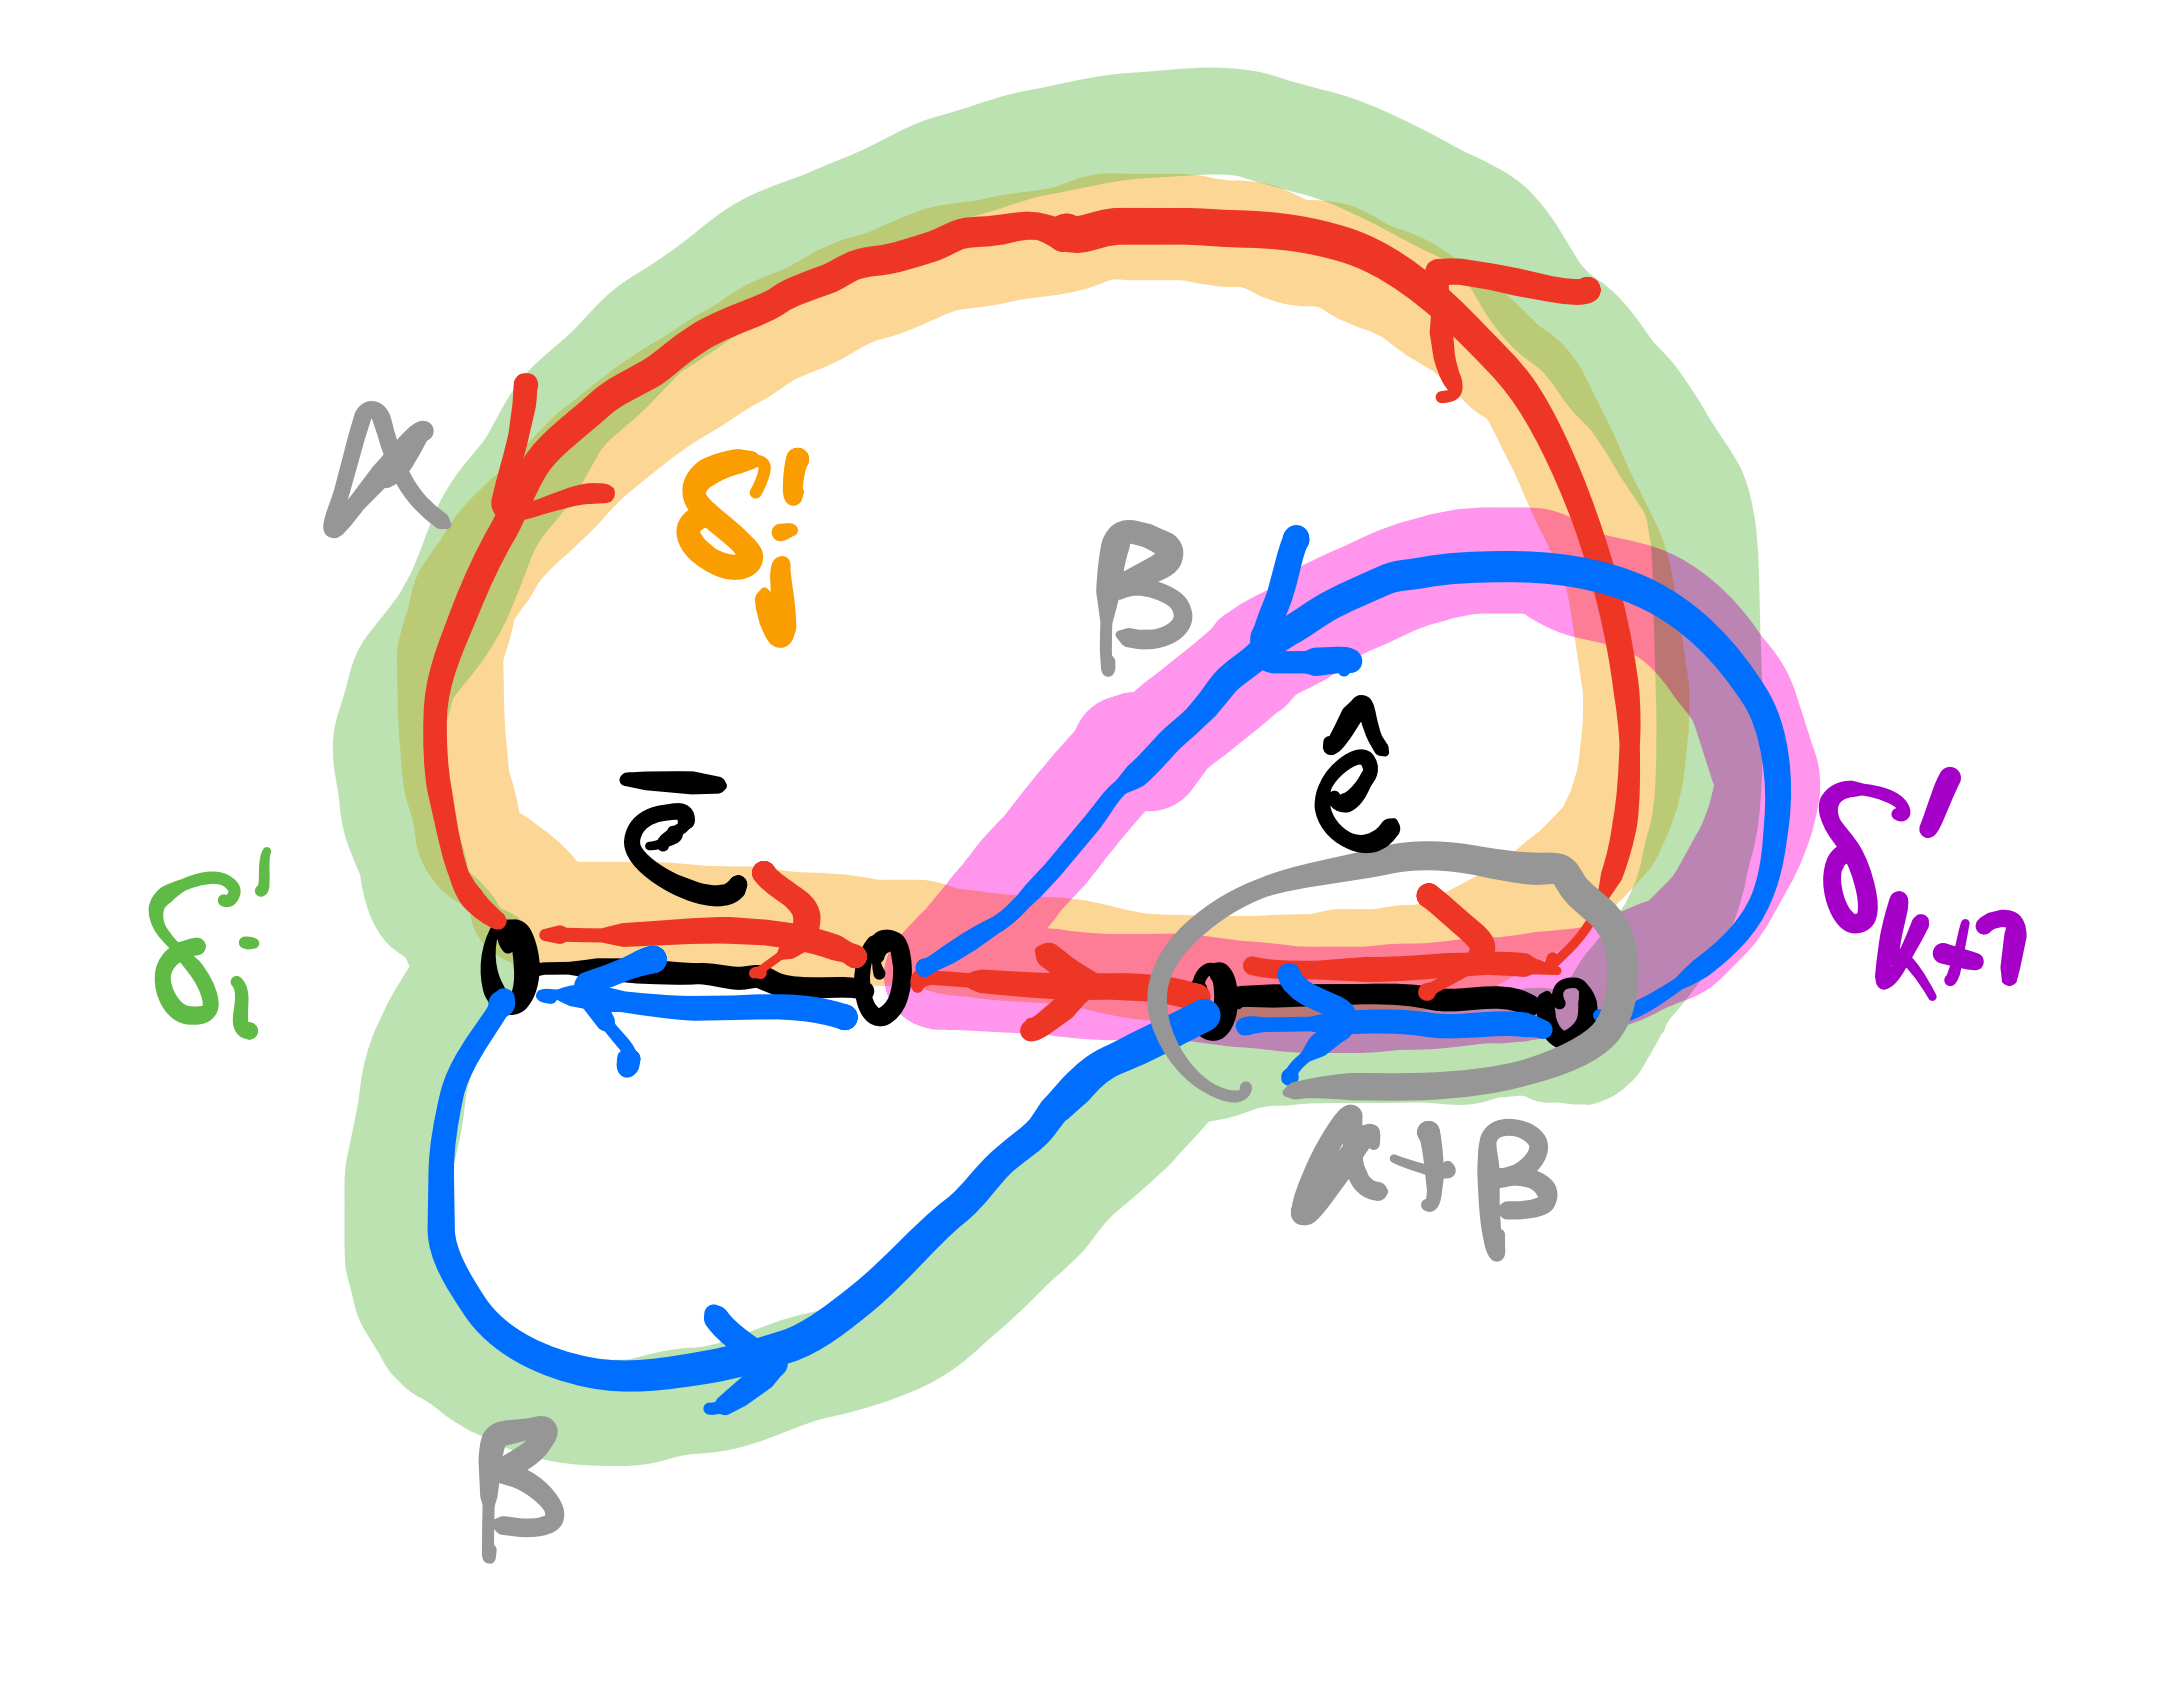
\includegraphics[width=\textwidth]{assignments/figures/cycle_decomposition2.png}
% \caption{Schematic illustration of the cycle flow update when parallel edges are present. $\vdelta_i$ sends $\alpha$ units of flow and $\vdelta_j$ sends $\beta$ units of flow. The net flow on the edge $\bar{e}$ is $\alpha - \beta$ and the net flow on the edge $\hat{e}$ is $\alpha + \beta$.}\label{fig:2:C:3:2}
% \end{marginfigure}

% Finally, if $\vdelta_i$ and $\vdelta_j$ share some parallel edges $\hat{E} \subseteq \Etil$, then we can find a new cycle decomposition consisting of more than two cycles. A schematic illustration is given in \cref{fig:2:C:3:2}. $\vdelta_i'$ and $\vdelta_j'$ are defined similarly to the previous case but accordingly to the edges as shown in the schematic illustration. We define the new cycle flow $\vdelta_{k'+1}'$ analogously routing $\beta$ units of flow. By the same arguments as in the previous case, $\vdelta_i' + \vdelta_j' + \vdelta_{k'+1}' = \vdelta_i + \vdelta_j$ and the new flows are not mutually antiparallel.

% It is easy to see that the schematic illustration also covers the case where $|\hat{E}| > 1$ and $|\bar{E}| > 1$, though we might need to add more cycles.
% \end{proof}

% We now describe an algorithm solving the undirected maximum flow problem. Suppose we are given the following subroutines: \begin{enumerate}
%     \item $\textsc{ComputeStep}(\Tilde{G}, \vf, \tau)$ that given the graph, $\vf \in \barrierflowset$, and a parameter $\tau > 1$ returns $\vdelta$ that is feasible for the update program \eqref{eq:2:update_program} and has $\norm{\mL_\vf\vdelta}_1 \leq 10 \cdot 2^\tau$. This algorithm takes time $T_{\textsc{ComputeStep}} \defeq 2^{\nicefrac{\log n}{\tau}} m$.
    
%     \item $\textsc{RoundFlow}(\vf)$ that given $\vf \in \barrierflowset$ with $\mB\vf = F(\vOne_t - \vOne_s)$ returns an integral flow $\hat{\vf}$ with $\hat{\vf}(\etil) = 0$, $-\vc(e) \leq \hat{\vf}(e) \leq \vc(e)$ for all $e \in E$, and $\mB\hat{\vf} = \hat{F}(\vOne_t - \vOne_s)$ where $\hat{F} \geq F - \vf(\etil) - 10$. This algorithm takes time $T_{\textsc{RoundFlow}} \defeq \TildeLandauO{m}$.
% \end{enumerate}

% \begin{algorithm}
%     \caption{\textsc{ComputeMaxFlow($G, s, t$)}}\label{alg:2}
%     $\vf \gets \vZero$\;
%     $\vf(\etil) \gets F$\;
%     \While{$\Phi(\vf) > -10m \log m$}{
%         $\vdelta \gets \textsc{ComputeStep}(\Tilde{G}, \vf, \tau)$\;
%         $\vf \gets \vf + \frac{1}{8\kappa^2}\vdelta$\;
%     }
%     $\hat{\vf} \gets \textsc{RoundFlow}(\vf)$\;
%     \While{$\val(\hat{\vf}) < F$}{
%         $\Tilde{\vf} \gets \textsc{FindAugmentingPath}(G_{\hat{\vf}}, s, t)$\;
%         $\hat{\vf} \gets \hat{\vf} + \Tilde{\vf}$\;
%     }
%     \Return{$\hat{\vf}$}
% \end{algorithm}

% \begin{thm}
% \Cref{alg:2} returns the maximum $s$-$t$ flow in the undirected graph $G$ in time $m^{2+o(1)}$.
% \end{thm}
% \begin{proof}
% We denote by $k$ the number of iterations of the first while-loop and by $\vf_i$ and $\vdelta_i$ the flow and update after/during the $i$-th iteration of said while-loop, respectively. We fix $\tau \defeq \log \log m$.\footnote{Throughout our analysis, we assume that the logarithm is with respect to base $2$.} We have, $\log \log m > \log \log 8 = \log 3 > 1$, where we used our assumption $m > 10$.

% Observe that $\vf_0$ (the flow before the first iteration of the while-loop) coincides with our characterization of $\vf_0$ in \cref{lem:initialization}, and hence, $\mB\vf_0 = F(\vOne_t - \vOne_s)$, $\vf_0 \in \barrierflowset$, and $\Phi(\vf_0) \leq 100 m \log m$.

% Let us assume $\vf_i \in \barrierflowset$. Per the definition of \textsc{ComputeStep}, $\mB\vdelta_{i+1} = \vZero$, $\trans{\grad\Phi_{\vf_i}}\vdelta_{i+1} = -1$, and $\norm{\mL_{\vf_i}\vdelta_{i+1}}_1 \leq 10 \cdot 2^\tau \eqdef \kappa$.\footnote{Note that $\kappa > 1$.} By \cref{lem:update}, it follows that $\mB\vf_{i+1} = F(\vOne_t - \vOne_s)$, $\vf_{i+1} \in \barrierflowset$, and \begin{align*}
%     \Phi(\vf_{i+1}) = \Phi\parentheses*{\vf_i + \frac{1}{8\kappa^2}\vdelta_{i+1}} \leq \Phi(\vf_i) - \frac{1}{16\kappa^2}.
% \end{align*} We have, \begin{align*}
%     \Phi(\vf_i) &= \Phi(\vf_0) + \sum_{j=1}^i \Phi(\vf_j) - \Phi(\vf_{j-1}) \\
%     &\leq 100 m \log m - \frac{i}{16\kappa^2} \margintag{using $\Phi(\vf_j) - \Phi(\vf_{j-1}) \leq -\nicefrac{1}{16\kappa^2}$}
% \end{align*} For any $0 \leq i < k$, the while-condition is satisfied, implying, \begin{align*}
%     &&-10 m \log m < \Phi(\vf_i) &\leq 100 m \log m - \frac{i}{16\kappa^2} \\
%     \implies&& \frac{i}{16\kappa^2} &< 110 m \log m \\
%     \implies&& i &= \LandauO{\kappa^2 m \log m}.
% \end{align*} In particular, \begin{align*}
%     k = \LandauO{\kappa^2 m \log m} = \LandauO{2^{2\tau} m \log m} = \LandauO{m \log^3 m} = m^{1+o(1)}.
% \end{align*}

% Evaluating $\textsc{RoundFlow}(\vf_k)$ yields a feasible integral flow $\hat{\vf}$ supported on $E$ routing $\hat{F}$ units of flow from $s$ to $t$, where \begin{align*}
%     \hat{F} &\geq F - \vf_k(\etil) - 10 \\
%     &\geq F - \frac{1}{m} - 10 \margintag{using \cref{lem:termination}} \\
%     &\geq F - 11.
% \end{align*}

% Finally, we find an augmenting path for $\hat{\vf}$ in the residual graph $G_{\hat{\vf}}$ until the flow is optimal (and no such augmenting path exists). As $\hat{\vf}$ and $\vc$ are integral, each augmenting path increases the value of the flow by at least one. As the initial $\hat{\vf}$ is almost optimal, we only have to find a constant number of augmenting paths. Each augmenting path can be found in $\LandauO{m}$ time using breadth-first search.

% The total runtime of \textsc{ComputeMaxFlow} is, \begin{align*}
%     &k \cdot T_{\textsc{ComputeStep}} + T_{\textsc{RoundFlow}} + \LandauO{m} \\
%     &= m^{2+o(1)} \cdot 2^{\frac{\log n}{\tau}} + \TildeLandauO{m} + \LandauO{m} \\
%     &= m^{2+o(1)} \cdot 2^{\frac{\log m}{\log \log m}} \margintag{using $n = \LandauO{m}$} \\
%     &= m^{2+o(1)+\frac{1}{\log \log m}} \\
%     &= m^{2+o(1)}. \qedhere
% \end{align*}
% \end{proof}

% \subsection{Part D: Stability}

% Finally, we will see that an update $\vdelta$ with small norm $\norm{\mL_\vf \vdelta}_1$ can only cause $\vl_{\vf + \vdelta}$ to change significantly in very few entries. This can be used to compute each individual update in time $m^{o(1)}$.

% We define $\vs \defeq \inv{\mL_\vf}\vl_{\vf + \vdelta}$ and $\mathcal{U} \defeq \{e \in \Etil \mid |\vs(e) - 1| > \nicefrac{1}{2}\}$.

% \begin{lem}
% If $\norm{\mL_\vf \vdelta}_1 \leq \nicefrac{1}{2}$, then $|\mathcal{U}| = \LandauO{1}$.
% \end{lem}
% \begin{proof}
% In the following, we will disregard whether $\etil \in \mathcal{U}$, as this only changes the size of $\mathcal{U}$ by a constant. By assumption, \begin{align*}
%     \sum_{e \in E} \vl_\vf(e) \cdot |\vdelta(e)| \leq \norm{\mL_\vf\vdelta}_1 \leq \frac{1}{2}.
% \end{align*} We have for all $e \in E$, \begin{align*}
%     \vs(e) = \frac{\vl_{\vf + \vdelta}(e)}{\vl_\vf(e)}.
% \end{align*} We will prove the following two claims.

% \begin{clm}\label{clm:2:D:1:1}
% For any $e \in E$, if $\vf(e) \geq 0$ and $|\vs(e) - 1| > \nicefrac{1}{2}$, then $|\vdelta(e)| > \frac{\vc(e) - \vf(e)}{3}$.
% \end{clm}
% \begin{clm}\label{clm:2:D:1:2}
% For any $e \in E$, if $\vf(e) < 0$ and $|\vs(e) - 1| > \nicefrac{1}{2}$, then $|\vdelta(e)| > \frac{\vc(e) + \vf(e)}{3}$.
% \end{clm}

% Using the two claims, we obtain, \begin{align*}
%     \sum_{e \in E} \vl_\vf(e) \cdot |\vdelta(e)| &= \sum_{\substack{e \in E \\ \vf(e) \geq 0}} \frac{|\vdelta(e)|}{\vc(e) - \vf(e)} + \sum_{\substack{e \in E \\ \vf(e) < 0}} \frac{|\vdelta(e)|}{\vc(e) + \vf(e)} \\
%     &> \frac{|\mathcal{U}|}{3},
% \end{align*} leading to a contradiction if $|\mathcal{U}| = \omega(1)$.
% \end{proof}

% First, observe that $|\vs(e) - 1| > \nicefrac{1}{2}$ iff either $\vs(e) < \nicefrac{1}{2}$ or $\vs(e) > \nicefrac{3}{2}$.

% \begin{proof}[Proof of \cref{clm:2:D:1:1}]
% Fix any $e \in E$ with $\vf(e) \geq 0$. We have, $\vl_\vf(e) = \vc(e) - \vf(e)$. We consider two cases: \begin{enumerate}
%     \item If $\vs(e) > \frac{3}{2}$, \begin{align*}
%         \frac{3}{2} < \vs(e) &= \frac{\vc(e) - \vf(e)}{\min\{\vc(e) - \vf(e) - \vdelta(e), \vc(e) + \vf(e) + \vdelta(e)\}} \\
%         &\leq \frac{\vc(e) - \vf(e)}{\vc(e) - \vf(e) - |\vdelta(e)|}
%     \end{align*} So, $|\vdelta(e)| > \frac{\vc(e) - \vf(e)}{3}$.
%     \item If $\vs(e) < \frac{1}{2}$, \begin{align*}
%         \frac{1}{2} > \vs(e) &= \frac{\vc(e) - \vf(e)}{\min\{\vc(e) - \vf(e) - \vdelta(e), \vc(e) + \vf(e) + \vdelta(e)\}} \\
%         &\geq \frac{\vc(e) - \vf(e)}{\vc(e) - \vf(e) - \vdelta(e)}
%     \end{align*} So, $\vdelta(e) < -\vc(e) + \vf(e) < 0$, and hence, $|\vdelta(e)| > \vc(e) - \vf(e)$. \qedhere
% \end{enumerate}
% \end{proof}

% \begin{proof}[Proof of \cref{clm:2:D:1:2}]
% Fix any $e \in E$ with $\vf(e) < 0$. We have, $\vl_\vf(e) = \vc(e) + \vf(e)$. We consider two cases: \begin{enumerate}
%     \item If $\vs(e) > \frac{3}{2}$, \begin{align*}
%         \frac{3}{2} < \vs(e) &= \frac{\vc(e) + \vf(e)}{\min\{\vc(e) - \vf(e) - \vdelta(e), \vc(e) + \vf(e) + \vdelta(e)\}} \\
%         &\leq \frac{\vc(e) + \vf(e)}{\vc(e) + \vf(e) - |\vdelta(e)|}
%     \end{align*} So, $|\vdelta(e)| > \frac{\vc(e) + \vf(e)}{3}$.
%     \item If $\vs(e) < \frac{1}{2}$, \begin{align*}
%         \frac{1}{2} > \vs(e) &= \frac{\vc(e) + \vf(e)}{\min\{\vc(e) - \vf(e) - \vdelta(e), \vc(e) + \vf(e) + \vdelta(e)\}} \\
%         &\geq \frac{\vc(e) + \vf(e)}{\vc(e) + \vf(e) + \vdelta(e)}
%     \end{align*} So, $\vdelta(e) > \vc(e) + \vf(e)$, and hence, $|\vdelta(e)| > \vc(e) + \vf(e)$. \qedhere
% \end{enumerate}
% \end{proof}

% \end{document}
